%%%%%%%%%%%%%%%%%%%%%%%%%%%%%%%%%%%%%%%%%%%%%%%%%%%%%%%%%%
%   Autoren:
%   Prof. Dr. Bernhard Drabant
%   Prof. Dr. Dennis Pfisterer
%   Prof. Dr. Julian Reichwald
%%%%%%%%%%%%%%%%%%%%%%%%%%%%%%%%%%%%%%%%%%%%%%%%%%%%%%%%%%

%%%%%%%%%%%%%%%%%%%%%%%%%%%%%%%%%%%%%%%%%%%%%%%%%%%%%%%%%%
%	ANLEITUNG: 
%   1. Ersetzen Sie firmenlogo.jpg im Verzeichnis img
%   2. Passen Sie alle Stellen im Dokument an, die mit 
%      @stud 
%      markiert sind
%%%%%%%%%%%%%%%%%%%%%%%%%%%%%%%%%%%%%%%%%%%%%%%%%%%%%%%%%%

%%%%%%%%%%%%%%%%%%%%%%%%%%%%%%%%%%%%%%%%%%%%%%%%%%%%%%%%%%
%	ACHTUNG: 
%   Für das Erstellen des Literaturverzeichnisses wird das 
%   modernere Paket biblatex in Kombination mit biber 
%   verwendet - nicht mehr das ältere Paket BibTex!
%
%   Bitte stellen Sie Ihre TeX-Umgebung entsprechend ein (z.B. TeXStudio): 
%   Einstellungen --> Erzeugen --> Standard Bibliographieprogramm: biber
%%%%%%%%%%%%%%%%%%%%%%%%%%%%%%%%%%%%%%%%%%%%%%%%%%%%%%%%%%

\documentclass[fontsize=12pt,BCOR=5mm,DIV=12,parskip=half,listof=totoc,
               paper=a4,toc=bibliography,pointlessnumbers]{scrreprt}
               
               %toc=listof,listof=entryprefix,
               
\makeindex

%% Elementare Pakete, Konfigurationen und Definitionen werden geladen (gegebenenfalls anpassen)
% !TEX root =  master.tex

%%%%%%%%%%%%%%%%%%%%%%%%%%%%%%%%%%%%%%%%%%%%%%%%%%%%%%%%%%%%%%%%%%
%	ANLEITUNG: 
% Passen Sie gegebenenfalls alle Stellen im Dokument an, die mit 
% @stud 
% markiert sind.
%%%%%%%%%%%%%%%%%%%%%%%%%%%%%%%%%%%%%%%%%%%%%%%%%%%%%%%%%%%%%%%%%%

%%
%% @stud
%%
%% LANGUAGE SETTINGS
\usepackage[ngerman]{babel} 	        % german language
\usepackage[german=quotes]{csquotes} 	% correct quoting using \enquote{}
%\usepackage[english]{babel}          % english language
%\usepackage{csquotes} 	              % correct quoting using \enquote{}

\usepackage{makeidx}                  % allows index generation
\usepackage{listings}	                %Format Listings properly
\usepackage{lipsum}                   % Blindtext
\usepackage{graphicx}                 % use various graphics formats
\usepackage[german]{varioref}         % nicer references \vref
\usepackage{caption}	                % better Captions
\usepackage{booktabs}                 % nicer Tabs
\usepackage[hidelinks=true]{hyperref} % keine roten Markierungen bei Links
\usepackage{fnpct}                    % Correct superscripts 
\usepackage{calc}                     % Used for extra space below footsepline, in particular
\usepackage{array}
\usepackage{acronym}
\usepackage{algorithm}
\usepackage{algpseudocode}
\usepackage{setspace}
\usepackage{tocloft}

%% Schriftarten- und Zeichenpakete
\usepackage[T1]{fontenc}
\usepackage[utf8]{inputenc}

%%
%% @stud
%%
%%	FONT SELECTION: Schriftarten und Schriftfamilie
%%%%%%%%%%%%%
%% SCHRIFTART
%%%%%%%%%%%%%
% 0) without decomment: normal font families 
% ...
% 1) Latin Modern 
\usepackage{lmodern}        
% 2) Times 
%\usepackage{mathptmx}         
% 3) Helvetica
%\usepackage[scaled=.92]{helvet} 
%%%%%%%%%%%%%%%%%%
%%	SCHRIFTFAMILIE
%%%%%%%%%%%%%%%%%%
% ohne Serifen
\renewcommand*{\familydefault}{\sfdefault}
\addtokomafont{disposition}{\sffamily}
%
% mit Serifen
%\renewcommand*{\familydefault}{\rmdefault}
%\addtokomafont{disposition}{\rmfamily}
%
% Typewriter
%\renewcommand*{\familydefault}{\ttdefault}
%\addtokomafont{disposition}{\ttfamily}

%%
%% @stud
%%
%% Uncomment the following lines to support hard URL breaks in bibliography 
%\apptocmd{\UrlBreaks}{\do\f\do\m}{}{}
%\setcounter{biburllcpenalty}{9000}% Kleinbuchstaben
%\setcounter{biburlucpenalty}{9000}% Großbuchstaben

%%
%% @stud
%%
%% FOOTNOTES: Count footnotes over chapters
%% \counterwithout{footnote}{chapter}

%	ACRONYMS
\makeatletter
\@ifpackagelater{acronym}{2015/03/20}
{\renewcommand*{\aclabelfont}[1]{\textbf{{\acsfont{#1}}}}}{}
\makeatother

%	LISTINGS
% @stud: ggf. Namen/Text anpassen (englisch)
\renewcommand{\lstlistingname}{Quelltext} 
\renewcommand{\lstlistlistingname}{Quelltextverzeichnis}
\lstset{numbers=left,
	numberstyle=\tiny,
	captionpos=b,
	basicstyle=\ttfamily\small}

%	ALGORITHMS
% @stud: ggf. Namen/Text anpassen (englisch)
\renewcommand{\listalgorithmname}{Algorithmenverzeichnis}
\floatname{algorithm}{Algorithmus}

%	PAGE HEADER / FOOTER
%	Warning: There are some redefinitions throughout the master.tex-file!  DON'T CHANGE THESE REDEFINITIONS!
\RequirePackage[automark]{scrlayer-scrpage}
%alternatively with separation lines: \RequirePackage[automark,headsepline,footsepline]{scrlayer-scrpage}

\renewcommand{\chaptermarkformat}{}
\RedeclareSectionCommand[beforeskip=0pt]{chapter}
\clearpairofpagestyles

%\ifoot[\rule{0pt}{\ht\strutbox+\dp\strutbox}DHBW Mannheim]{\rule{0pt}{\ht\strutbox+\dp\strutbox}DHBW Mannheim}
\ofoot[\rule{0pt}{\ht\strutbox+\dp\strutbox}\pagemark]{\rule{0pt}{\ht\strutbox+\dp\strutbox}\pagemark}
\ohead{\headmark}

\newcommand{\TitelDerArbeit}[1]{\def\DerTitelDerArbeit{#1}\hypersetup{pdftitle={#1}}}
\newcommand{\AutorDerArbeit}[1]{\def\DerAutorDerArbeit{#1}\hypersetup{pdfauthor={#1}}}
\newcommand{\Firma}[1]{\def\DerNameDerFirma{#1}}
\newcommand{\Kurs}[1]{\def\DieKursbezeichnung{#1}}
\newcommand{\Abteilung}[1]{\def\DerNameDerAbteilung{#1}}
\newcommand{\Studiengangsleiter}[1]{\def\DerStudiengangsleiter{#1}}
\newcommand{\WissBetreuer}[1]{\def\DerWissBetreuer{#1}}
\newcommand{\FirmenBetreuer}[1]{\def\DerFirmenBetreuer{#1}}
\newcommand{\Bearbeitungszeitraum}[1]{\def\DerBearbeitungszeitraum{#1}}
\newcommand{\Abgabedatum}[1]{\def\DasAbgabedatum{#1}}
\newcommand{\Matrikelnummer}[1]{\def\DieMatrikelnummer{#1}}
\newcommand{\Studienrichtung}[1]{\def\DieStudienrichtung{#1}}
\newcommand{\ArtDerArbeit}[1]{\def\DieArtDerArbeit{#1}}
\newcommand{\Literaturverzeichnis}{Literaturverzeichnis}

\newcommand{\settingBibFootnoteCite}{
	\setlength{\bibparsep}{\parskip}		  % Add some space between biblatex entries in the bibliography
	\addbibresource{bibliography.bib}	    % Add file bibliography.bib as biblatex resource
	\DefineBibliographyStrings{ngerman}{andothers = {{et\,al\adddot}},}
}

\newcommand{\setTitlepage}{
	% !TEX root =  master.tex
% @stud: ggf. Namen/Text anpassen (englisch)
\begin{titlepage}
\begin{minipage}{\textwidth}
		\vspace{-2cm}
		\noindent \hfill 
\includegraphics{\imagedir/logo.jpg}
\end{minipage}
\vspace{1em}
%\sffamily
\begin{center}
	{\textsf{\large Duale Hochschule Baden-W\"urttemberg Mannheim}}\\[4em]
	{\textsf{\textbf{Integrationsseminar}}}\\[6mm]
	{\textsf{\textbf{\Large{}\DerTitelDerArbeit}}} \\[1.5cm]
	{\textsf{\textbf{\large{}Studiengang Wirtschaftsinformatik}}\\[6mm]
	\textsf{\textbf{Studienrichtung \DieStudienrichtung}}}\vspace{15em}
	
	\begin{minipage}{\textwidth}
		\begin{tabbing}
		Wissenschaftliche(r) Betreuer(in): \hspace{0.85cm}\=\kill
		Verfasser: \> \DerAutorDerArbeit \\[1.5mm]
		Matrikelnummer: \> \DieMatrikelnummer \\[1.5mm]
%		Firma: \> \DerNameDerFirma  \\[1.5mm]
%		Abteilung: \> \DerNameDerAbteilung \\[1.5mm]
		Kurs: \> \DieKursbezeichnung \\[1.5mm]
		Studiengangsleiter: \> \DerStudiengangsleiter \\[1.5mm]
		Dozent: \> \DerWissBetreuer \\[1.5mm]
%		Firmenbetreuer(in): \> \DerFirmenBetreuer \\[1.5mm]
		Bearbeitungszeitraum: \> \DerBearbeitungszeitraum\\[1.5mm]
%		alternativ:\\[1.5mm]
%		Eingereicht: \> \DasAbgabedatum	
		\end{tabbing}
	\end{minipage}
\end{center}
\end{titlepage}
	\pagenumbering{roman} % Römische Seitennummerierung
	\normalfont	
}

\newcommand{\initializeText}{
	\clearpage
	\ihead{\chaptername~\thechapter} % Neue Header-Definition
	\pagenumbering{arabic}           % Arabische Seitenzahlen
}

\newcommand{\initializeBibliography}{
	\ihead{}
	\printbibliography[title=\Literaturverzeichnis] 
	\cleardoublepage
}

\newcommand{\initializeAppendix}{
	\appendix
  \ihead{}
  \cftaddtitleline{toc}{chapter}{Anhang}{}
}



%%
%% @stud
%%
%% PERSÖNLICHE ANGABEN (BITTE VOLLSTÄNDIG EINGEBEN zwischen den Klammern: {...})
%%
%\ArtDerArbeit{Seminar} % "Bachelor" oder "Projekt" wählen
\TitelDerArbeit{OS Scheduling Algorithmen}
\AutorDerArbeit{Jannik Völker, Benedikt Prisett, Eric Echtermeyer}
%\Abteilung{<Ihre Abteilung>}
%\Firma{<Ihre Firma>}
\Kurs{WWI-21-DSA}
\Studienrichtung{Data Science}
% TODO 
\Matrikelnummer{, 5370226, 6373947}
\Studiengangsleiter{Prof. Dr.-Ing. habil. Dennis Pfisterer}
\WissBetreuer{Prof. Dr. Maximilian Scherer}
%\FirmenBetreuer{<Ihr(e) Firmenbetreuer(in)>}
\Bearbeitungszeitraum{13.11.2023 -- 07.02.2024}
%\Abgabedatum{11.01.2024}

%%
%% @stud
%%
%% BIBLIOGRAPHY (@stud: Bibliographie-Stil wählen - Position und Indizierung)
%%  Auswahl zwischen: 
%%   NUMERIC Style
%%   IEEE Style
%%   ALPHABETIC Style
%%   HARVARD Style
%%   CHICAGO Style 
%%   (oder eigenen zulässigen Stil wählen) 
%%
%%%%%%%%%%%%%
%% Zitierstil
%%%%%%%%%%%%%
% NUMERIC Style - e. g. [12]
\newcommand{\indextype}{numeric} 
%
% IEEE Style - numeric kind of style 
%\newcommand{\indextype}{ieee} 
%
% ALPHABETIC Style - e. g. [AB12]
%\newcommand{\indextype}{alphabetic} 
%
% HARVARD Style 
%\newcommand{\indextype}{apa} 
%
% CHICAGO Style 
%\newcommand{\indextype}{authoryear}
%
%%%%%%%%%%%%%%%%%%%%%%
%% Position des Zitats
%%%%%%%%%%%%%%%%%%%%%%
\newcommand{\position}{inline} 
%
% (!!) FOOTNOTE POSITION NOT RECOMMENDED IN MINT DOMAIN:
%\newcommand{\position}{footnote}

%% Final: Setzen des Zitierstils und der Zitatposition
\usepackage[backend=biber, autocite=\position, style=\indextype, sorting=none]{biblatex}
\settingBibFootnoteCite

%%
%% Definitionen und Commands
%%
\newcommand{\abs}{\par\vskip 0.2cm\goodbreak\noindent}
\newcommand{\nl}{\par\noindent}
\newcommand{\mcl}[1]{\mathcal{#1}}
\newcommand{\nowrite}[1]{}
\newcommand{\NN}{{\mathbb N}}
\newcommand{\imagedir}{img}

\makeindex

\begin{document}

\setTitlepage

%%%%%%%%%%%%%%%%%%%%%%%%%%%%%%%%%%%
% EHRENWÖRTLICHE ERKLÄRUNG
%
% @stud: ewerkl.tex bearbeiten
%
%% !TEX root =  master.tex
\clearpage
\chapter*{Ehrenwörtliche Erklärung}

% Wird die folgende Zeile auskommentiert, erscheint die ehrenwörtliche
% Erklärung im Inhaltsverzeichnis.

% \addcontentsline{toc}{chapter}{Ehrenwörtliche Erklärung}
Ich versichere hiermit, dass ich die vorliegende Seminararbeit mit dem Titel ``\textit{\DerTitelDerArbeit}'' selbstständig verfasst und 
keine anderen als die angegebenen Quellen und Hilfsmittel benutzt habe. Ich versichere zudem, dass die eingereichte elektronische 
Fassung mit der gedruckten Fassung übereinstimmt.

\vspace{3cm}
Ort, Datum \hfill \DerAutorDerArbeit
 
%\cleardoublepage  
%%%%%%%%%%%%%%%%%%%%%%%%%%%%%%%%%%%

%%%%%%%%%%%%%%%%%%%%%%%%%%%%%%%%%%%
% SPERRVERMERK
%
% @stud: nondisclosurenotice.tex bearbeiten
%
%% !TEX root =  master.tex
\chapter*{Sperrvermerk}

\begin{center}
\fbox{
		\begin{minipage}{33em}
			\textbf{Ein Sperrvermerk sollte nur bei berechtigtem Bedarf gesetzt werden!\\[10pt] 
				Beachten Sie, dass mit Sperrvermerk	versehene Arbeiten nicht für weitere wissenschaftliche Zwecke 
				außerhalb des Firmenkontextes oder zur Publikation verwendet werden dürfen.\\[10pt]
				Wir empfehlen, wenn m\"oglich, auf den Sperrvermerk zu verzichten.\\[10pt]
				Besprechen Sie diese Problematik mit Ihrer Firma!}
		\end{minipage}
}
\end{center}

(Mustertext) Der Inhalt dieser Arbeit darf weder als Ganzes noch in Auszügen Personen außerhalb des Prüfungsprozesses 
und des Evaluationsverfahrens zugänglich gemacht werden, sofern keine anders lautende Genehmigung der Ausbildungsstätte vorliegt. 

\cleardoublepage
 
%\cleardoublepage
%%%%%%%%%%%%%%%%%%%%%%%%%%%%%%%%%%%

%%%%%%%%%%%%%%%%%%%%%%%%%%%%%%%%%%%
%	KURZFASSUNG
%
% @stud: acknowledge.tex bearbeiten
%
%% !TEX root =  master.tex
\chapter*{Danksagung}

Hier können Sie eine Danksagung schreiben. 



%\cleardoublepage 
%%%%%%%%%%%%%%%%%%%%%%%%%%%%%%%%%%%

%%%%%%%%%%%%%%%%%%%%%%%%%%%%%%%%%%%
% VERZEICHNISSE und ABSTRACT
%
% @stud: ggf. nicht benötigte Verzeichnisse auskommentieren/löschen
%
\tableofcontents
\cleardoublepage

% Abbildungsverzeichnis
\phantomsection
\addcontentsline{toc}{chapter}{\listfigurename}
\listoffigures
\cleardoublepage

%	Tabellenverzeichnis
%\phantomsection
%\addcontentsline{toc}{chapter}{\listtablename}
%\listoftables
%\cleardoublepage

%	Listingsverzeichnis / Quelltextverzeichnis
%\lstlistoflistings
%\cleardoublepage

% Algorithmenverzeichnis
%\listofalgorithms
%\cleardoublepage

% Abkürzungsverzeichnis
% @stud: acronyms.tex bearbeiten
% !TEX root =  master.tex
\clearpage
\chapter*{Abkürzungsverzeichnis}	
\addcontentsline{toc}{chapter}{Abkürzungsverzeichnis}

\begin{acronym}[XXXXXXX]
	\acro{OS}{Betriebssystem}	
	\acro{cpu}[CPU]{Central Processing Unit}
	\acro{FCFS}{First Come First Serve}
	\acro{FIFO}{First-In-First-Out}
	\acro{MLQ}{Multilevel-Queue}
	\acro{cfs}[CFS]{Completely Fair Scheduler}
	\acro{eevdf}[EEVDF]{Earliest Eligible Virtual Deadline First}
\end{acronym} 
\cleardoublepage

%	Kurzfassung / Abstract
% @stud: abstract.tex bearbeiten
%% !TEX root =  master.tex
\chapter*{Kurzfassung (Abstract)}
\addcontentsline{toc}{chapter}{Kurzfassung (Abstract)}

Hier können Sie die Kurzfassung (engl.~Abstract) der Arbeit schreiben. Beachten Sie dabei die Hinweise zum Verfassen der Kurzfassung.


 
%\cleardoublepage

%%%%%%%%%%%%%%%%%%%%%%%%%%%%%%%%%%%%%%%%%%%%%%%%%%%%%%%%%%%%%%%%%%%%%%%%%%%%%%%%%%%%%%%%%%
% KAPITEL UND ANHÄNGE
%
% @stud:
%   - nicht benötigte: auskommentieren/löschen
%   - neue: bei Bedarf hinzufügen mittels input-Kommando an entsprechender Stelle einfügen
%%%%%%%%%%%%%%%%%%%%%%%%%%%%%%%%%%%%%%%%%%%%%%%%%%%%%%%%%%%%%%%%%%%%%%%%%%%%%%%%%%%%%%%%%%

\initializeText
\onehalfspacing

%%%%%%%%%%%%%%%%%%%%%%%%%%%%%%%%%%%
% KAPITEL
%
% @stud: einzelne Kapitel bearbeiten und eigene Kapitel hier einfügen
%
% Einleitung
%% !TEX root =  master.tex
\chapter{Einleitung}

\nocite{*}

Dieses Kapitel enthält die Einleitung mit ihren verschiedenen Abschnitten/Sections und Unterabschnitten.

\section{Beispiel Abschnitt: \LaTeX-Installation}

Zur Verwendung von \LaTeX-Installation einer Distribution z.~B.~TeXLive, MikTex etc.~sowie eines Editors z.~B.~TeXStudio, TeXnicCenter etc.~notwendig.

Installieren Sie zun\"achst die Distribution und anschließend den Editor. Beim ersten Start des Editors \"offnet sich ein 
Konfigurationsassistent, der zun\"achst nach dem Pfad der installierten Distribution fragt. 

Nach der Installation können k\"onnen Einstellungen z.~B.~f\"ur einen PostScript-Viewer gemacht werden. 
Dieser Schritt kann ohne Weiteres \"ubersprungen werden. Entscheidend sind die Einstellungen f\"ur den pdf-Viewer. 

Jetzt kann \LaTeX~verwendet werden. Um die Ausgabe eines Dokumentes zu erzeugen, muss das Dokument kompiliert werden (Ausgabe >
Aktives Dokument > Erstellen und betrachten).

\subsection{Beispiel Unterabschnitt: Aufbau eines \LaTeX-Dokuments}

Ein \LaTeX-Dokument besteht in der Regel aus folgenden Komponenten:
\begin{itemize}
	\item Pr\"aambel
	\item Titelseite
	\item Textteil
\end{itemize}

\subsection{Beispiel Unterabschnitt auf zweiter Ebene: Pr\"aambel}
In der Pr\"aambel werden global die Einstellungen f\"ur das gesamte Dokument definiert. Hierbei k\"onnen z.~B.~die Seitenr\"ander, 
der Zeilenabstand oder auch die Sprache f\"ur die Silbentrennung festgelegt werden. In der ersten Zeile eines jeden Dokumentes wird dabei
immer die zu verwendende Klasse festgelegt. Standardm\"aßig kann hier die Artikel-Klasse gew\"ahlt werden:

\texttt{\textbackslash documentclass[12pt,titlepage]\{article\}}

In den eckigen Klammern wird dabei u.a. die Standardschriftgr\"o\ss e f\"ur das gesamte Dokument festgelegt. 

Au\ss erdem werden in der Pr\"aambel die f\"ur das Dokument ben\"otigten Pakete festgelegt. Gebr\"auchlich sind vor allem folgende Pakete:
{\texttt{
\begin{itemize}
	\item \textbackslash usepackage[ngerman]\{babel\}
	\item \textbackslash usepackage[latin1]\{inputenc\}
	\item \textbackslash usepackage\{color\}
	\item \textbackslash usepackage[a4paper]\{geometry\}
	\item \textbackslash usepackage\{amssymb\}
	\item \textbackslash usepackage\{amsthm\}
	\item \textbackslash usepackage\{graphicx\}
\end{itemize}
}

Im vorliegenden Fall werden die Pakete in der Konfigurationsdatei \texttt{config.tex} festgelegt, deren Inhalt durch 
\texttt{\textbackslash input\{config\}} in das Hauptdokument \texttt{master.tex} inkludiert wird.

\subsubsection{Beispiel Unterabschnitt auf zweiter Ebene: Titelseite}

Nachdem die Dokumenten-Klasse und die zu verwendenden Pakete festgelegt worden sind,
folgt die Titelseite. Da die Titelseite bereits Teil des eigentlichen Dokuments ist, muss ihr
unbedingt der Befehl \texttt{\textbackslash begin\{document\}} vorausgehen. Am Ende des Dokuments sollte der Befehl
\texttt{\textbackslash end\{document\}} gesetzt werden. Alles was nach diesem Befehl steht, wird vom Compiler nicht mehr beachtet.

\section{Noch ein Beispiel-Abschnitt}

Der Textteil beinhaltet nun den eigentlichen Text des Dokuments.


% mehrere Grundlagen- und Forschungs-Kapitel

% !TEX root =  master.tex

\chapter{Grundlagen der Visualisierung}
% Einleitung
Das Ziel dieses Projektes liegt in der Erstellung eines hochwertigen Lehrvideos, um den komplexen Sachverhalt der Scheduling Algorithmen von Betriebssystemen intuitiv darzustellen, sodass interessierte Zuschauer relevante Sachverhalte schnell verstehen können. Um für den Lernenden ein Lehrvideo mit möglichst hoher Qualität anbieten zu können, ist eine Beschäftigung mit theoretischen Grundlagen der Visualisierung, den Animationen und anderen Aspekten der Audio und Farbgestaltung unabdingbar. Daher wird im folgenden auf grundlegende Theorien in einer Literaturrecherche eingegangen, welche direkt in das von uns produzierten Lehrvideo eingebracht werden. 

% Bestätigung für Animationsvideo mit kurzem Disclaimer
Unsere Herangehensweise ein Lehrvideo zu erstellen, wird durch die Dual-Coding-Theorie von Allan Paivio bestätigt, welche besagt, dass Informationen besser verarbeitet und erinnert werden können, wenn diese sowohl visuell als auch verbal aufbereitet werden \autocite{paivio_dual_1991}. Dies ist ein Kernaspekt von Lehrvideos und wird umgestzt, indem neben visuellen Darstellungen wie Diagrammen oder animierten Algorithmen diese stets zugleich auf der Tonspur erklärt werden. Laut der Cognitive Load Theorie von John Sweller ist hierbei allerdings darauf zu achten, dass die kognitive Belastung des Lernenden berücksichtigt wird. Um ein effektives Lehrvideo zu erstellen, ist es entscheidend, eine Ausgewogenheit zwischen informativen Inhalten und überladenen Darstellungen zu finden \autocite{sweller_cognitive_2011}. 
Animationen können hierbei helfen komplexe Konzepte in einfach zu verstehende visuelle Elemente zu zerlegen, wodurch die kognitive Belastung reduziert werden kann. Um den Lernenden hierbei jedoch nicht kognitiv zu überlasten, ist es essentiell, dass Animationen stets passend und synchron zu der Tonspur angeordnet sind und diese beiden Komponenten nicht voneinander abweichen. Sollte dies doch der Fall sein, kann Verwirrtheit oder eine kognitiver Leistungsüberschreitung des Lernenden entstehen, wodurch die vermittelten Inhalte nicht zielgerichtet aufgenommen werden können \autocite{sweller_cognitive_2011}. 

% Möglichkeit Überforderung zu vermeiden
Eine Möglichkeit diese kognitive Überlastung zu vermeiden, ist die Anwendung der Multimedia Prinzipien von Richard E. Mayer. Dieser erarbeitete, dass eine angemessene Kombination von Text, Bildern und Animationen das Lernen deutlich verbessern kann, da Lehrinhalte hierduch prägnanter dargestellt werden können \autocite{mayer_multimedia_2002}. Insbesondere das Kontiguitätsprinzip, welches besagt, dass verbundene Text- und Bildinformationen zeitlich und räumlich nahe präsentiert werden sollten, ist für die Gestaltung von Bildungsanimationen relevant. Durch einen dezent animierten Text können grafische Vorgänge parallel zur Tonspur beschrieben werden. Der Lernende kann sich diesen Text nun im eigenen Tempo durchlesen ohne bei einer kurzen Unaufmerksamkeit das Verständnis für den gesamten Sachverhalt zu verlieren. Da es sich hierbei um ein zentrales Prinzip handelt, wird dieses innerhalb unseres Lehrvideos ebenfalls zahlreich umgesetzt. 

% Screenshot einfügen mit Beschreibung. Etwas mit Grafik & animiertem Text dazu
\begin{figure}[h]
	\centering
	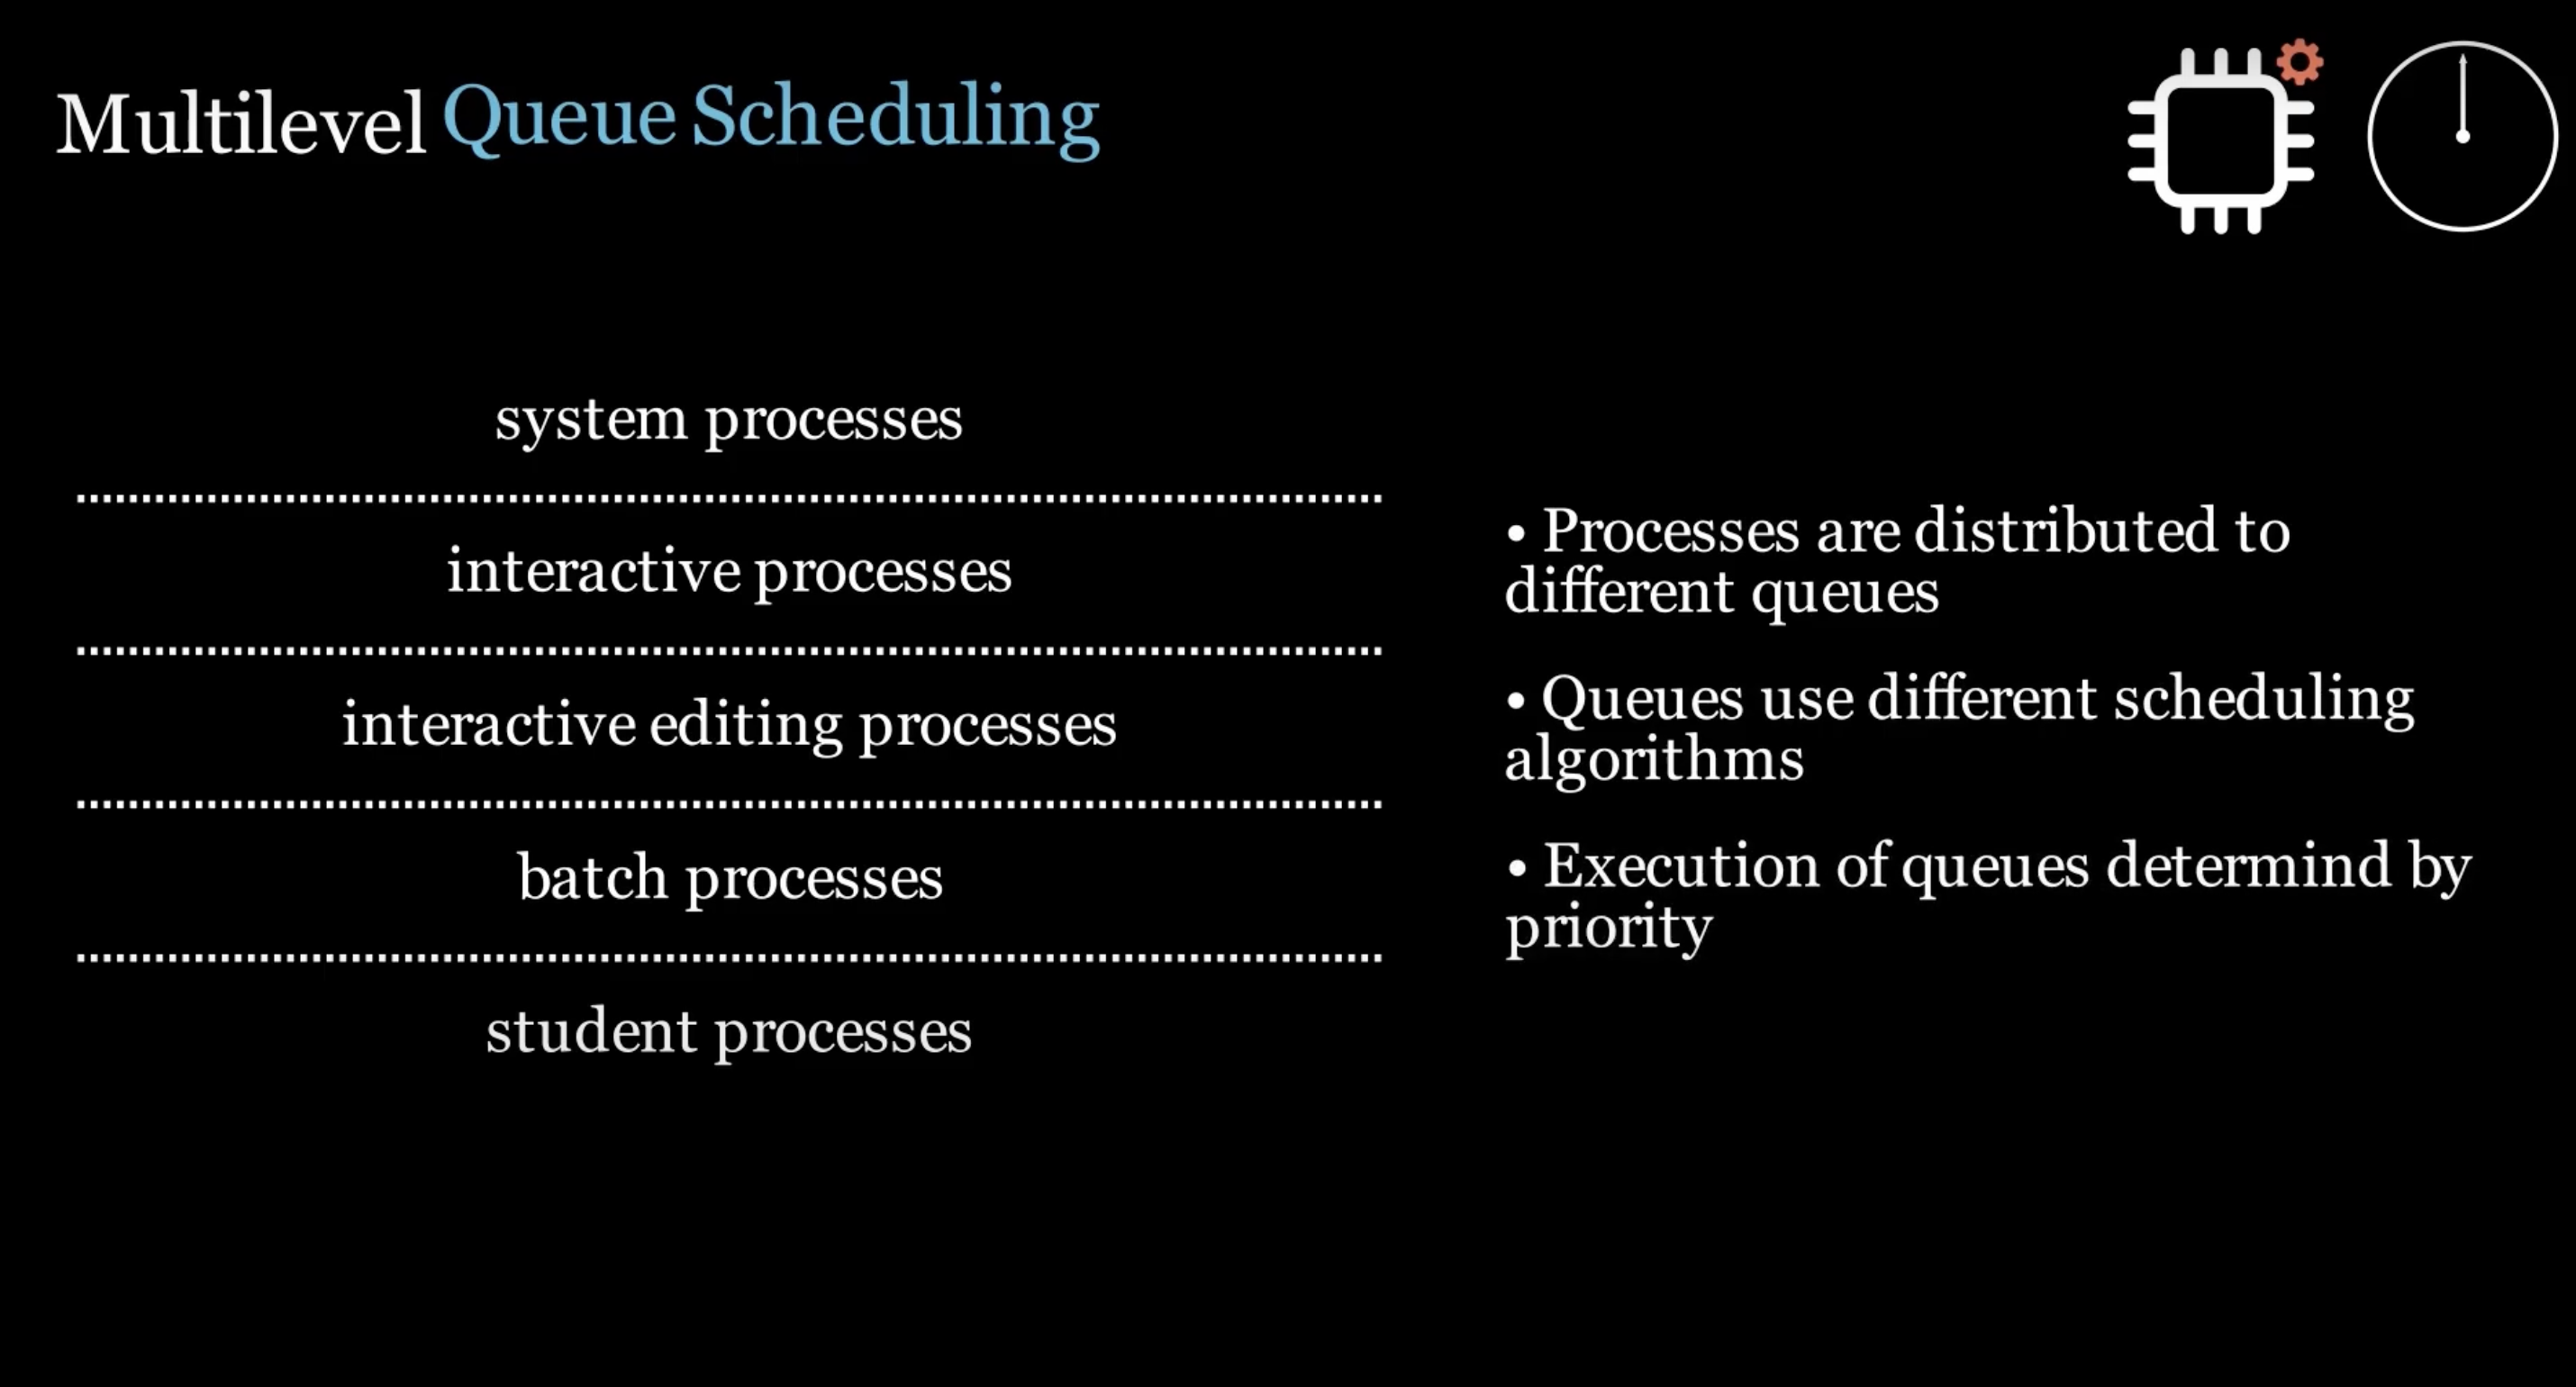
\includegraphics[width=0.8\linewidth]{img/screen_text.png} 
	\caption{Die Szene zur Erklärung des \ac{MLQ}-Algorithmus zeigt die Kombination zwischen animierten Bildinformationen mit unterstützendem Text.}
	\label{fig:screen_text} 
\end{figure}

% Komposition von Objekten
Des Weiteren bietet die Gestaltpsychologie von Kurt Koffka wertvolle Einsichten zur visuellen Wahrnehmung, insbesondere wie Menschen visuelle Informationen verarbeiten und interpretieren \autocite{koffka_principles_1999}. So spielt die Hierarchie visueller Elemente eine entscheidende Rolle, indem diese das Hervorheben wichtiger Inhalte ermöglicht und die Aufmerksamkeit des Lernenden gezielt lenken kann. Die Führung des Blicks durch eine durchdachte Komposition und die strategische Verwendung von Leerflächen können ebenfalls dazu beitragen, die kognitive Belastung zu minimieren und die Aufnahme der Lerninhalte zu erleichtern \autocite{koffka_principles_1999}.
Indem diese beispielhaft genannten Prinzipien berücksichtigt werden, können Lehrvideos nicht nur ästhetsich ansprechend sein, sondern auch die Lernprozesse durch eine verbesserte visuelle Wahrnehmung unterstützen. Beispielsweise werden die Funktionsweisen der unterschiedlichen Scheduling Algorithmen innerhalb unseres Lehrvideos durch sich bewegende Prozesse dargestellt, welche durch eine sich drehende \ac{cpu} abgearbeitet werden. Dies unterstützt dem Zuschauer Zusammenhänge leichter und schneller zu verstehen. 

Auch die Gestaltprinzipien der Wahrnehmung von Max Wertheimer, welche von der Gestaltpsychologie abzugrenzen sind, bieten Einsichten für die Gestaltung von Bildungsanimationen \autocite{wertheimer_untersuchungen_2017}. Diese Prinzipien, wie die Gruppierung von Elementen nach Nähe oder Ähnlichkeit, können genutzt werden, um Beziehungen und Strukturen zu verdeutlichen. So kann beispielsweise das Prinzip der Nähe dazu verwendet werden, um zu zeigen, wie verschiedene Elemente miteinander in Beziehung stehen. 

% Screenshot einfügen mit Beschreibung. Etwas mit Grafik & animiertem Text dazu
\begin{figure}[h]
	\centering
	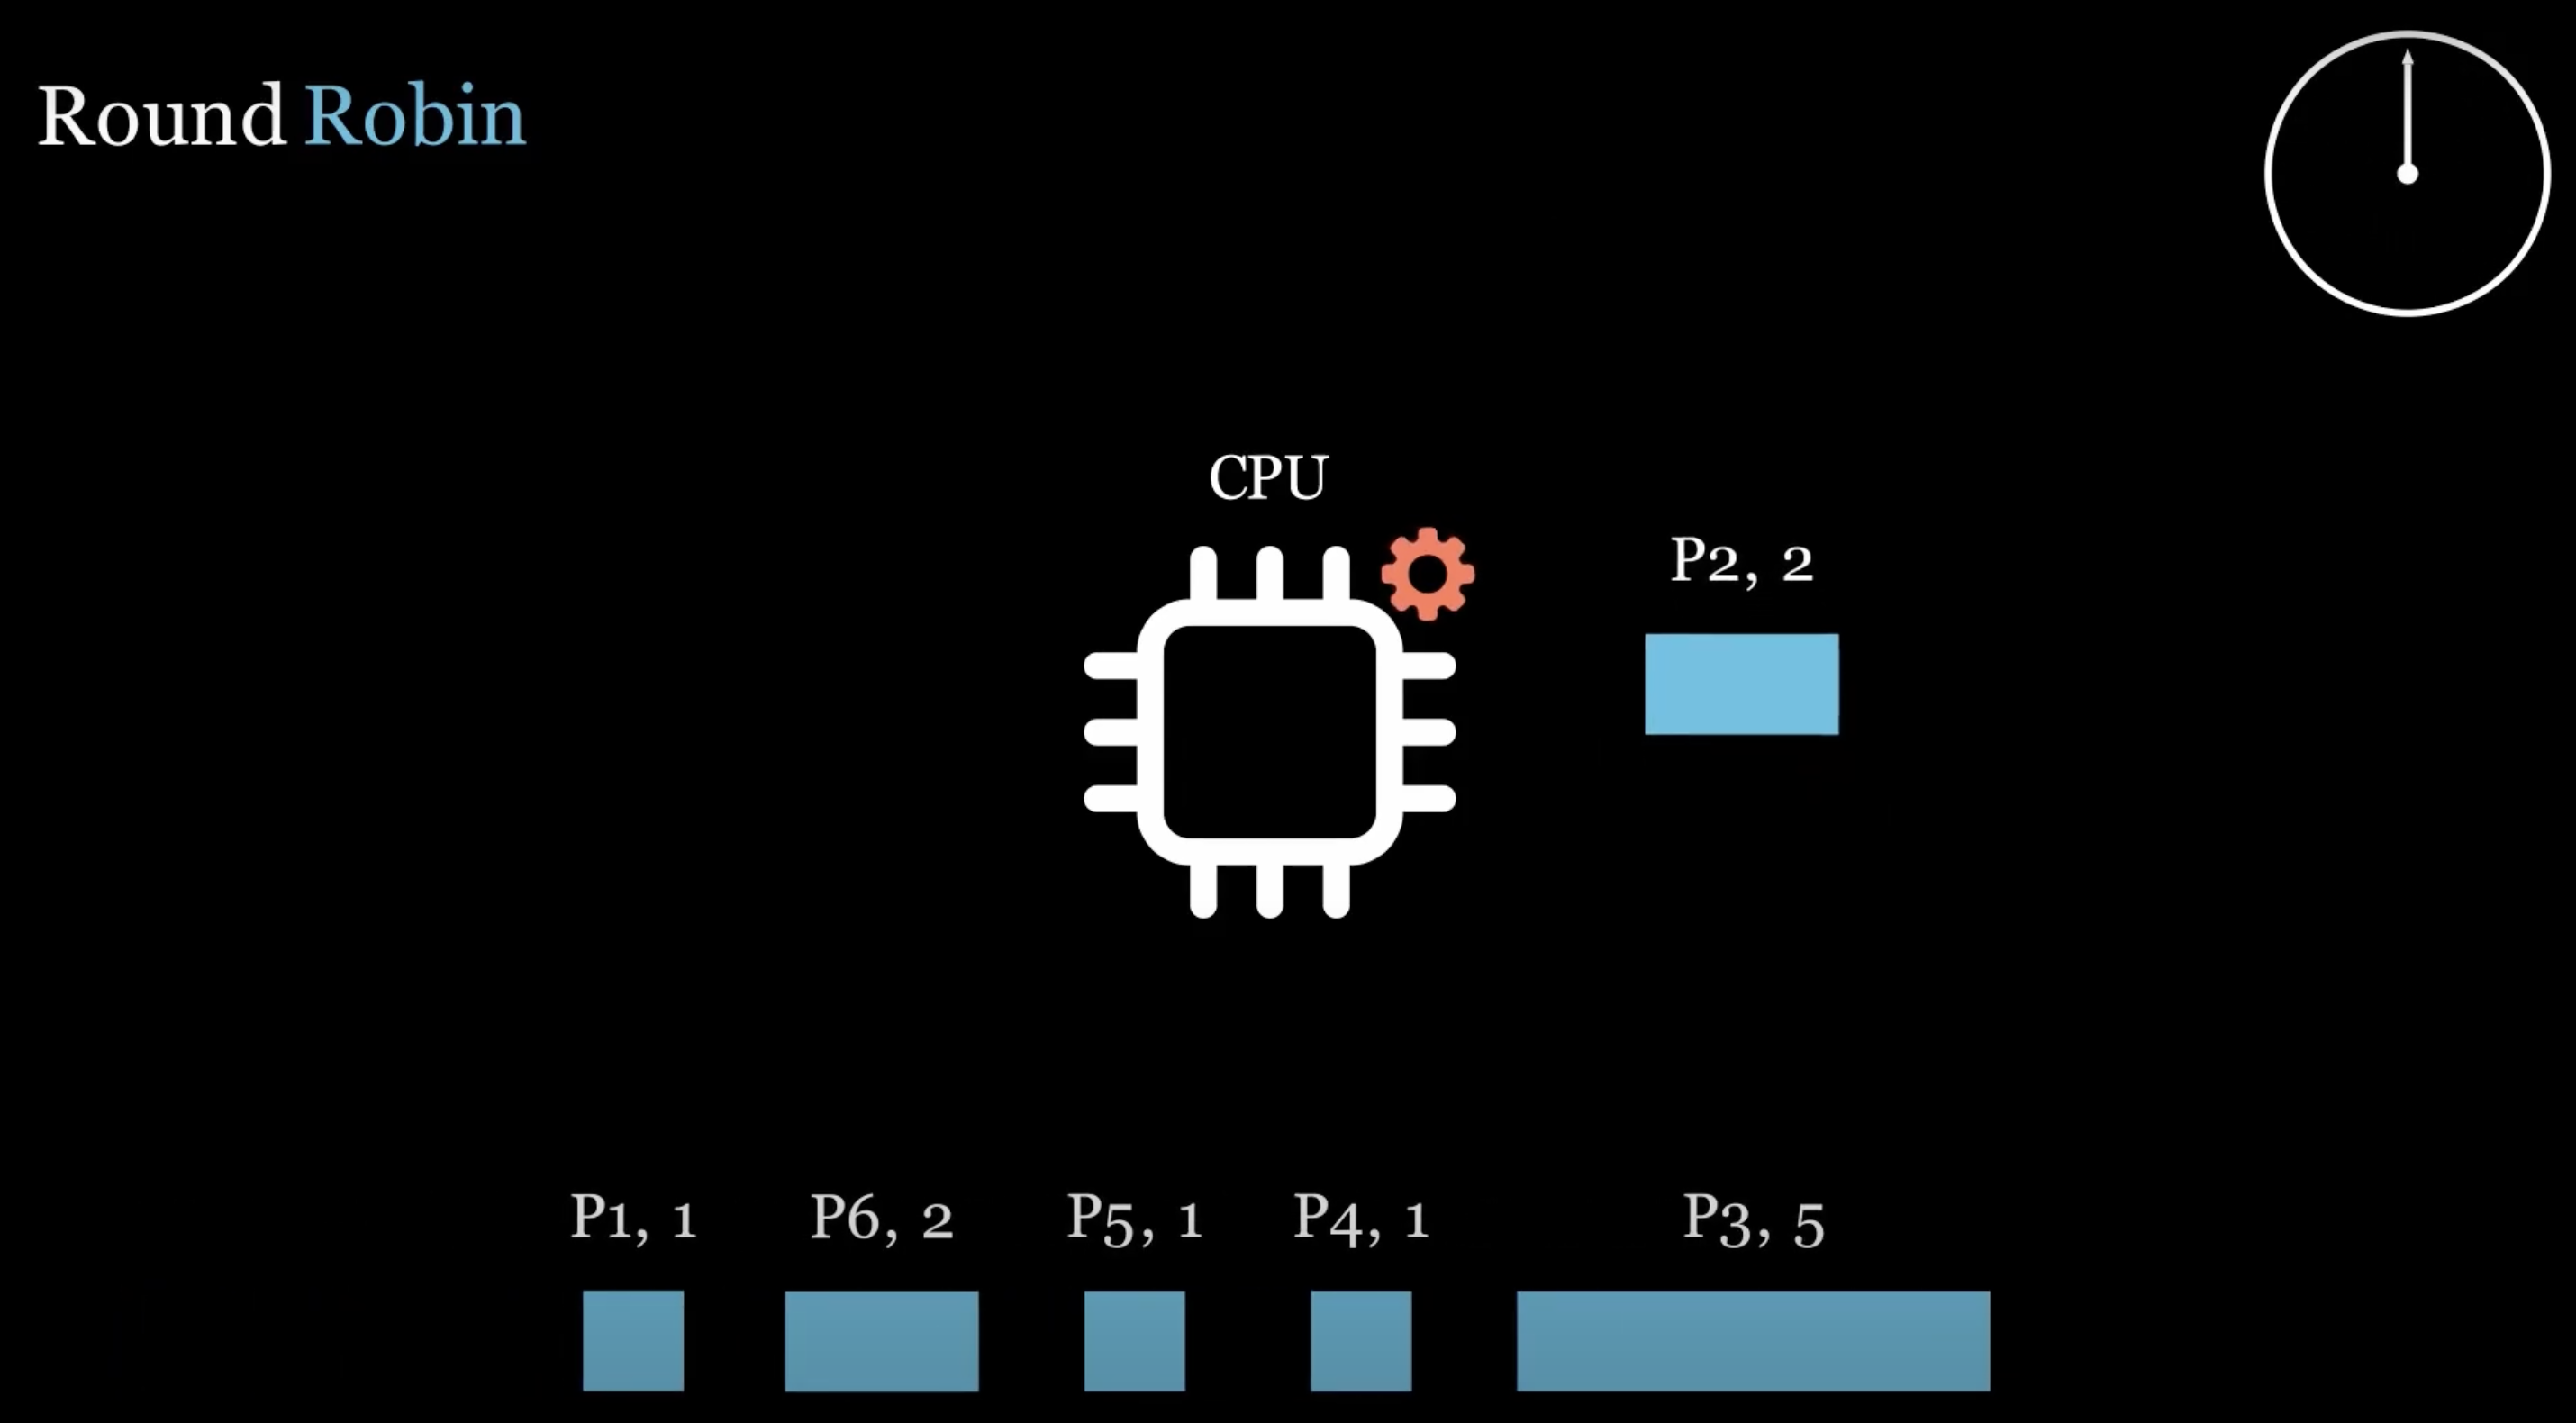
\includegraphics[width=0.8\linewidth]{img/screen_komposition.png} 
	\caption{Wird ein Prozess von der \ac{cpu} abgearbeitet, reduziert sich die Breite des Prozesses, um eine Verringerung der verbleibenden Bearbeitungszeit darzustellen.}
	\label{fig:screen_komposition} 
\end{figure}


%\textbf{Farbgestaltung}:
Neben der Wichtigkeit von Animationen und Komposition ist eine geschickte Auswahl der gewählten Farben ebenso essentiell. Laut der Farbtheorie kann die Auswahl von Farben und Kontrasten dabei unterstützen, wichtige Informationen hervorzuheben und die visuelle Erfahrung, und somit die vermittelten Inhalte, der Lernenden zu bereichern \autocite{ballard_art_1964}. Das von uns erstellte Lehrvideo versucht eine konsistente farbliche Harmonie zu bewirken, was durch die kontinuierliche Verwendung einer abgestimmten Farbpalette erreicht wird. Teilweise werden zudem wichtige Komponenten mithilfe von Sekundärfarben hervorgehoben, wie beispielsweise in Abbildung \ref{fig:screen_farben} das Erscheinen eines neuen Prozesses durch die Farbe orange betont wird. 

% Screenshot einfügen von "Animation". Wie ein Algorithmus etwas verarbeitet oder so
\begin{figure}[h]
	\centering
	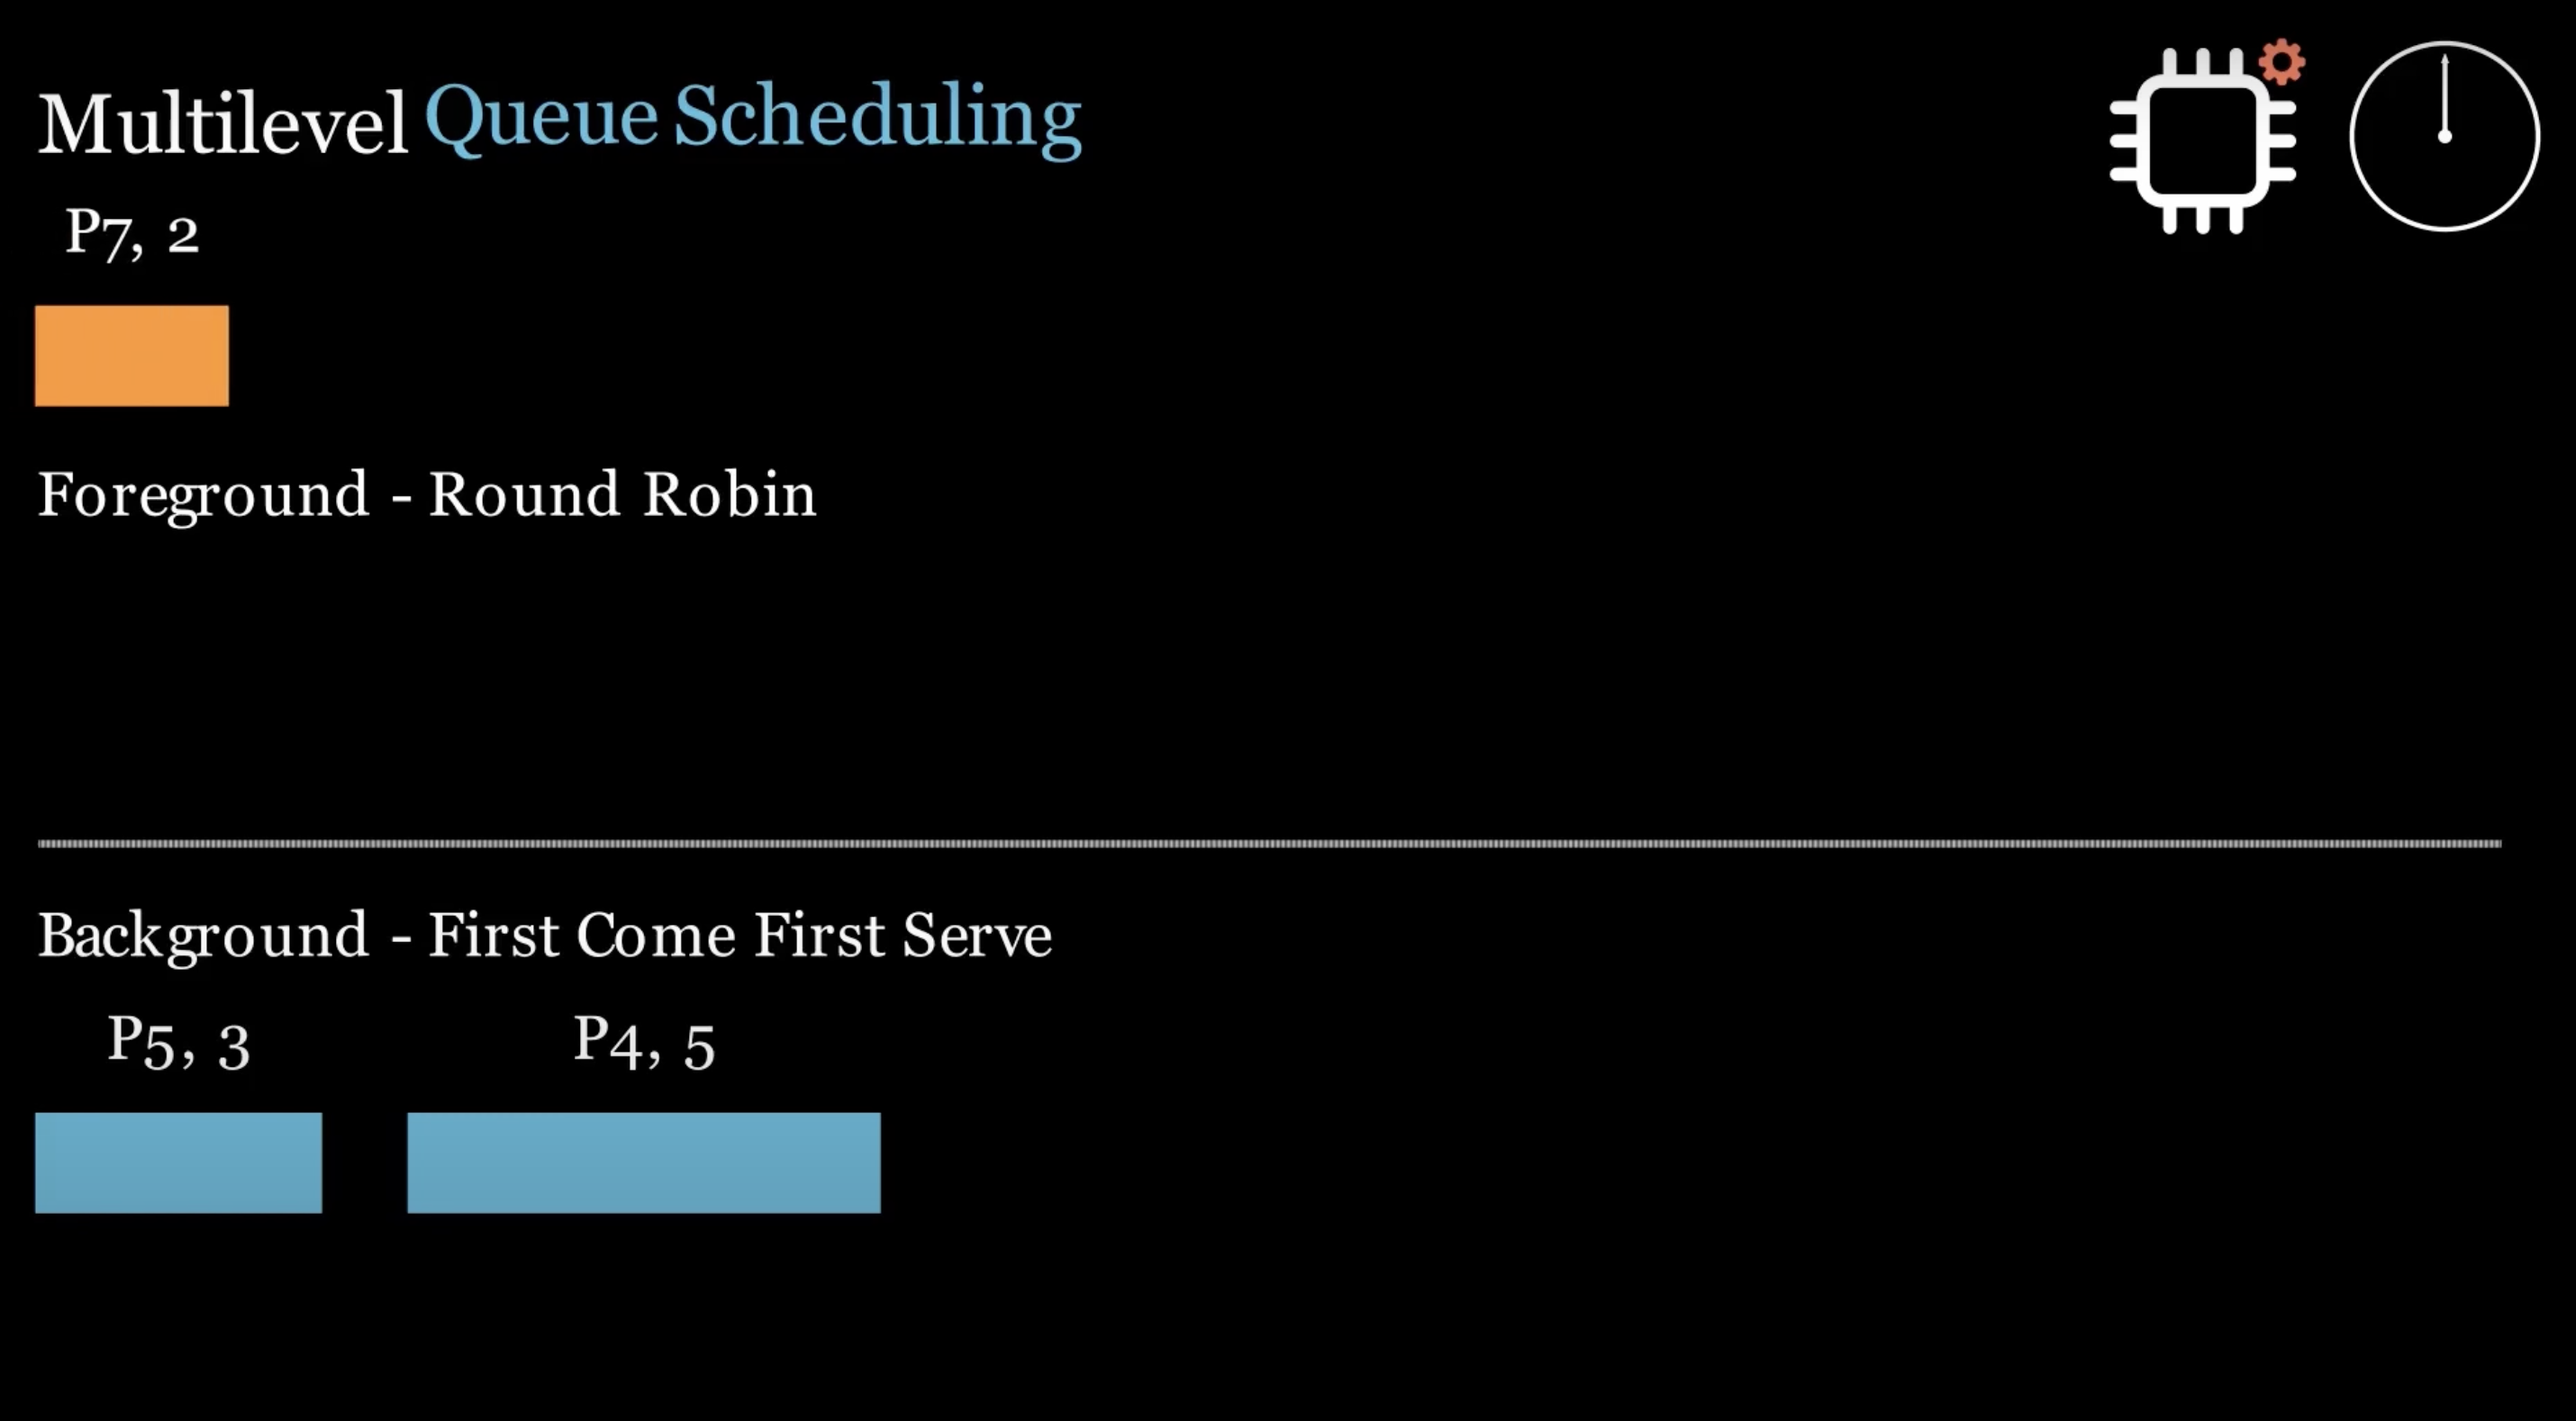
\includegraphics[width=0.8\linewidth]{img/screen_farben.png} 
	\caption{In der \ac{MLQ} Szene wird ein neu hinzukommender Prozess mithilfe einer orangenen Farbe für den Lernenden hervorgehoben.}
	\label{fig:screen_farben} 
\end{figure}


%\textbf{Auditive Unterstützung}:
Abgesehen der zuvor beschriebenen visuellen Komponenten nimmt die Musik ebenfalls eine zentrale Rolle ein, da diese entscheidend zur Steigerung der Aufmerksamkeit, zur Steuerung der Stimmung und zur Verbesserung des Verständnis beitragen kann. John A. Sloboda betont in "The Musical Mind: The Cognitive Psychology of Music", dass Musik und Soundeffekte nicht nur die emotionale Reaktion der Zuschauer beeinflussen, sondern auch deren Engagement und Erinnerungsvermögen fördern können \autocite{sloboda_musical_1986}. Durch den gezielten Einsatz von Musik können bestimmte Stimmungen erzeugt oder verstärkt werden, was die Aufnahme und Verarbeitung von Informationen unterstützt. Ebenso können Soundeffekte dazu dienen, wichtige Momente hervorzuheben und den Lernenden dazu anzuregen, ihre volle Aufmerksamkeit auf spezifische Aspekte des Videos zu richten \autocite{sloboda_musical_1986}. 
So versucht unser Lehrvideo mit einer ansprechenden und beruhigenden audiovisellen Erlebnis die kognitive Verarbeitungsfähigkeit der Lernenden zu fördern und ein effektiveres Lernerlebnis zu bieten. 


%\textbf{Storyline und Stringenz}:
Nachdem nun visuelle und auditive Aspekte beschrieben wurden, ist die Erwähnung anderer Aspekte wie der Integration von Storytelling innerhalb des Lehrvideos essentiell. Auch wenn es sich hierbei nicht um eine Art der Visualisierung handelt, kann hierduch eine eine emotionale Verbindung zum Lehrmaterial hergestellt werden, worduch dieses zugänglicher und einprägsamer wird. Roger C. Schank unterstreicht in "Tell me a story: A new look at real and artificial memory" die Relevanz von Geschichten auf das menschliche Verständnis und Erinnerungsvermögen \autocite{schank_tell_1990}. Indem Lehrvideos eine solche narrative Stringenz aufweisen, bei welcher beispielsweise die Optimierung einer ToDo-Liste durch den Einsatz eines Betriebssystem-Scheduling-Algorithmus als durchgängige Story dient, kann das Interesse und die Motivation der Zuschauer gesteigert werden. Die in unserem Lehrvideo dargestellte ToDo-Liste enthält hierbei bewusst Einträge, welche eine persönliche Relevanz für den Zuschauer haben, um eine emotionale Verbindung herzustellen. Durch diesen Ansatz wird zu Beginn und am Ende des Videos nicht nur die Aufmerksamkeit gefesselt, sondern es wird auch ein Rahmen geschaffen, der das Verständnis und die Merkfähigkeit der vermittelten Inhalte maßgeblich verbessert.


\begin{figure}[h]
	\centering
	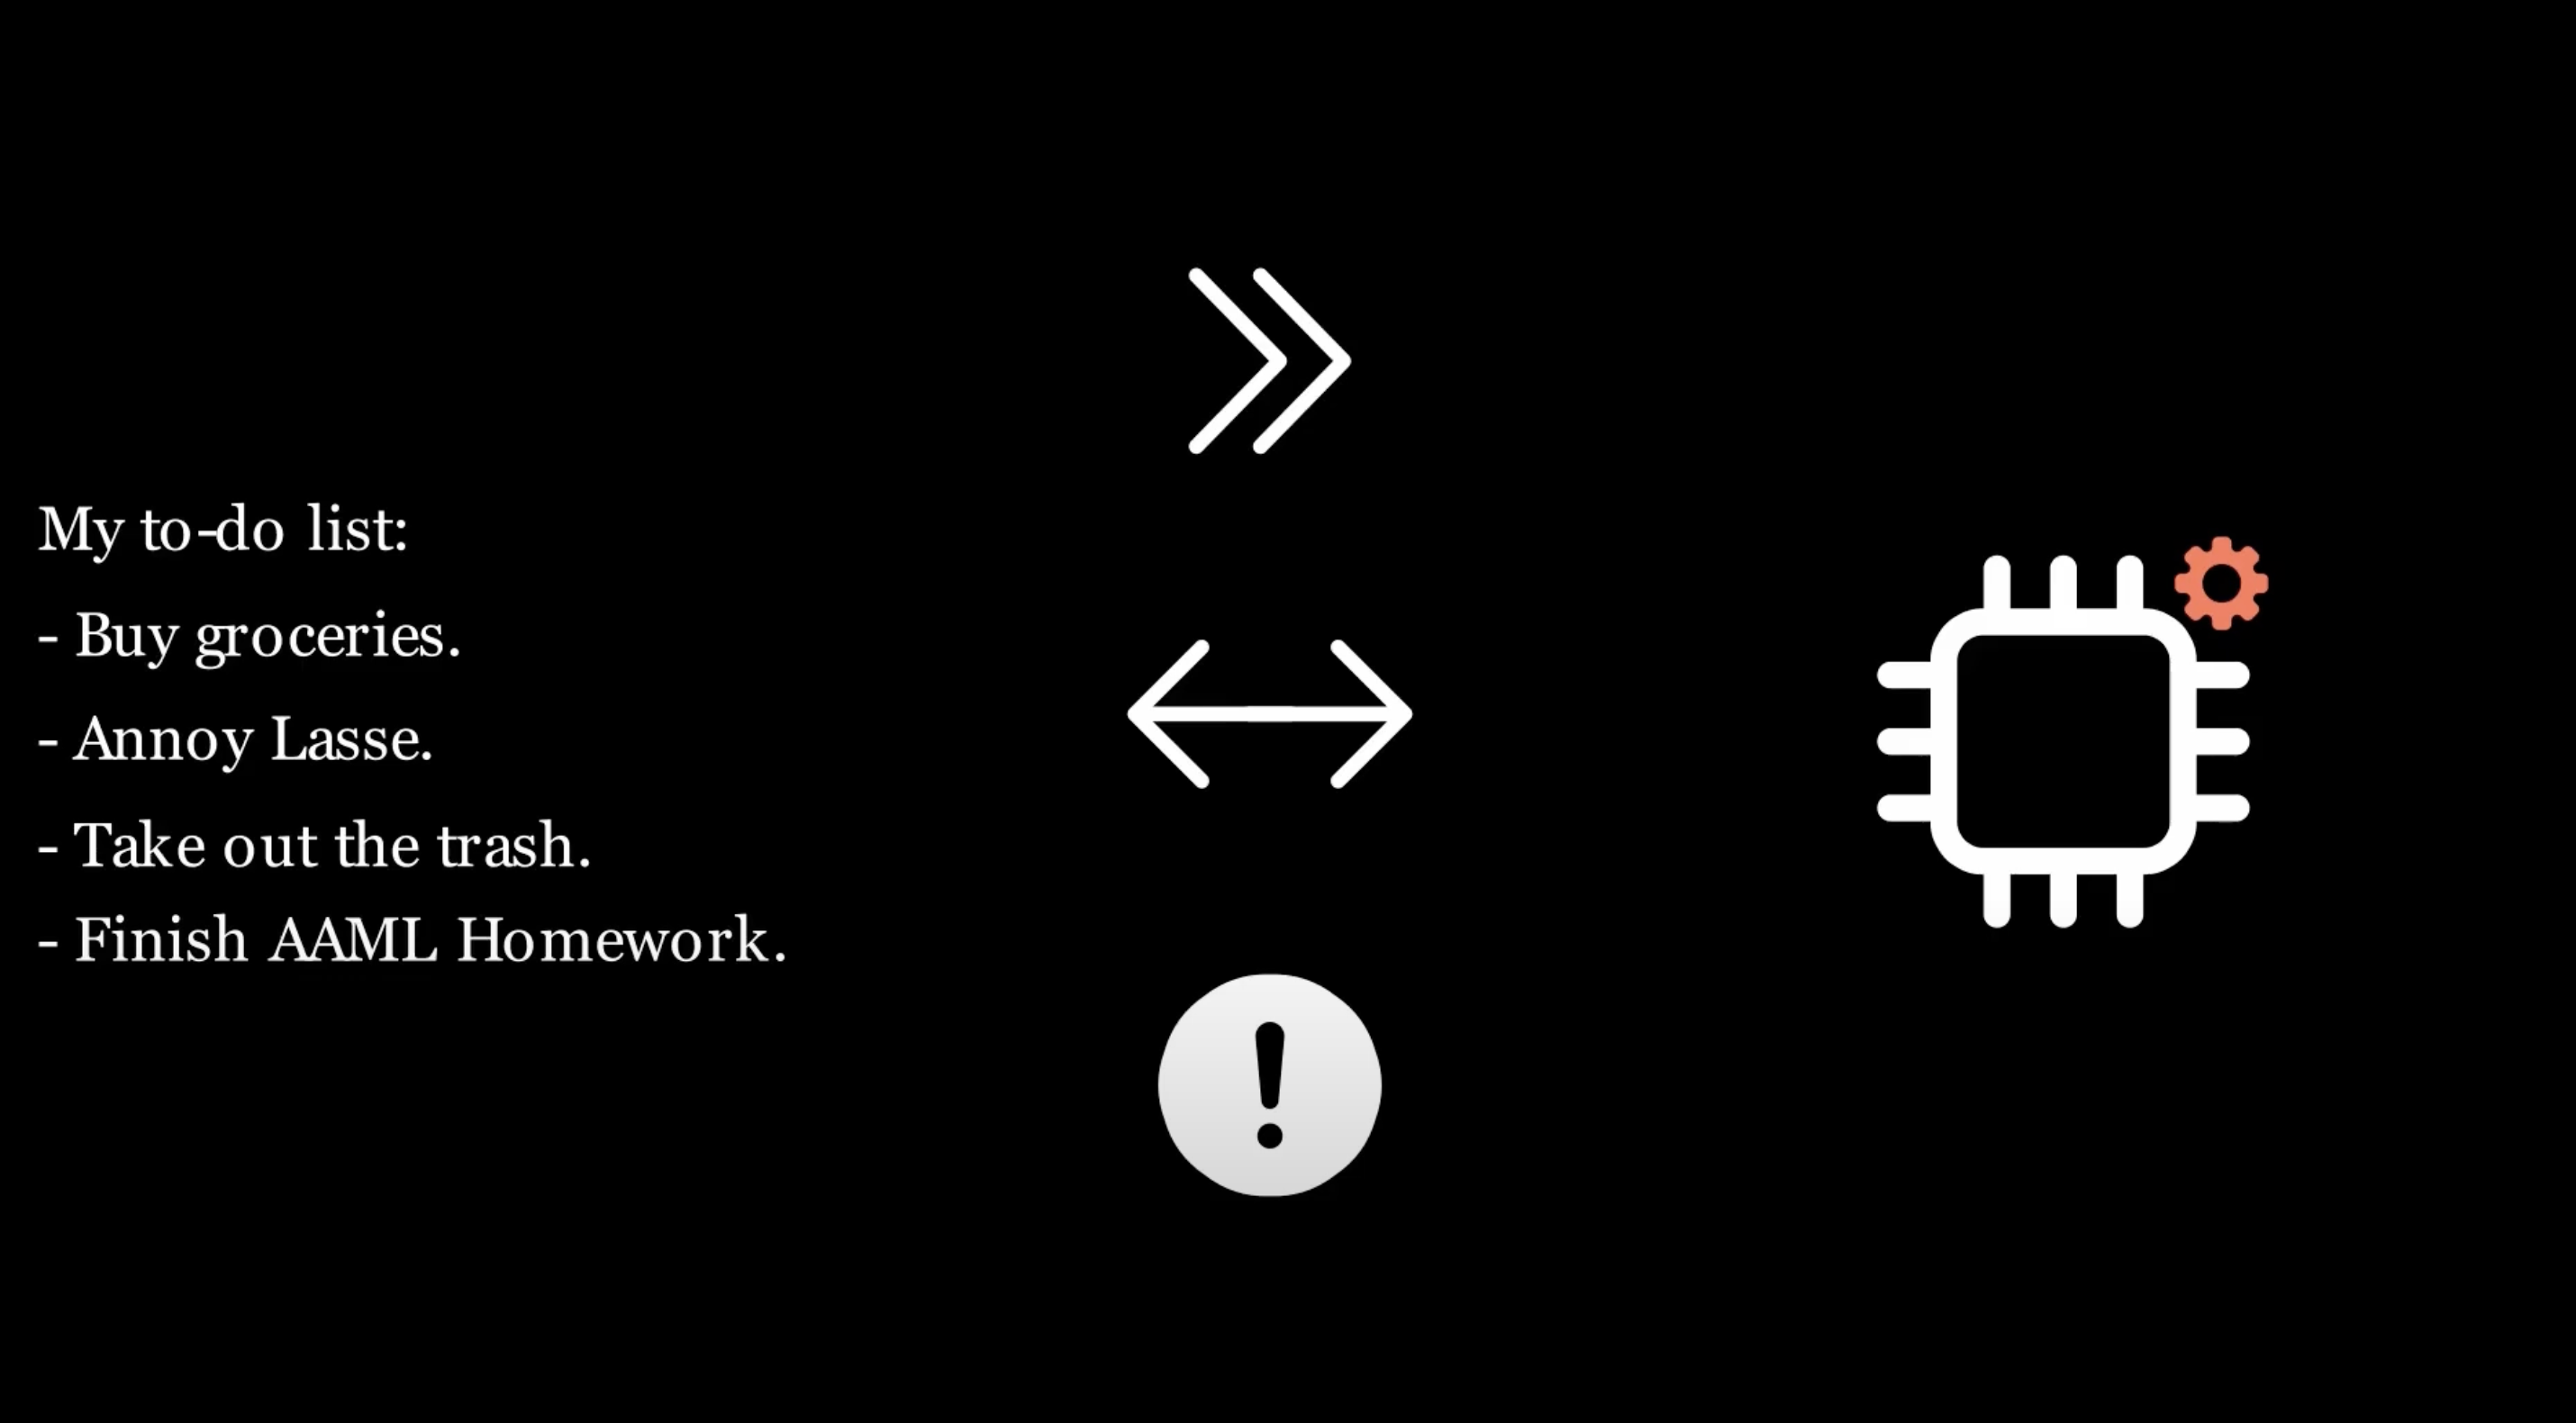
\includegraphics[width=0.8\linewidth]{img/screen_todo.png} 
	\caption{Die ToDo Liste dient als Einleitung und Abschluss des Lehrvideos, um eine inhaltliche Stringenz zu bewirken.}
	\label{fig:screen_todo} 
\end{figure}


Nachdem nun auf die theoretischen Grundlagen der Visualisierung eingegangen wurde, beschäftigen sich die folgenden Kapitel mit der Erklärung verwendeter Scheduling Algorithmen und einer anschließenden Performance Analyse dieser im Vergleich.


\input{01_1_section_visualiserung}

% !TEX root =  master.tex
\chapter{OS Scheduling Algorithmen}
Das Kernstück eines jeden modernen Betriebssystems is dessen Fähigkeit eine Vielzahl von Prozessen effizient und effektiv zu verwalten. Diese Prozessverwaltung, auch bekannt als Scheduling, ist eine komplexe Aufgabe, welche darüber entscheidet, welcher Prozess zu welchem Zeitpunkt von der \ac{CPU} verarbeitet wird. Da moderne Betriebssysteme stets eine hohe Anzahl von Hintergrundprozessen bis hin zu anspruchsvollen Anwendungen verarbeiten müssen, ist die Verwendung leistungsfähiger OS Scheduling Algorithmen essentiell. Im folgenden werden drei unterschiedliche Algorithmen des OS Scheduling vorgestellt, mit aufsteigender Komplexität. Jeder dieser Algorithmen hat eigenen Stärken und Schwächen, die ihn für bestimmte Szenarien und Anforderungen geeignet machen. Von den einfachen, aber grundlegenden Ansätzen wie First Come First Serve bis hin zu komplexeren Strategien wie Multilevel Queue Scheduling, spiegelt die Entwicklung dieser Algorithmen die Fortschritte in der Computertechnologie und unser zunehmendes Verständnis von effizientem Prozessmanagement wider.

% !TEX root =  master.tex

\section{First-Come-First-Serve}

Einer der grundlegenden Scheduling-Algorithmen für Betriebssysteme ist \ac{FCFS}, auch bekannt als \ac{FIFO}. \ac{FCFS} verarbeitet eingehende Prozesse in der Reihenfolge ihres Eintreffens, wobei der zuerst eingetroffene Prozess zuerst abgearbeitet wird. Ein Prozess wird so lange von der \ac{cpu} bearbeitet, bis er vollständig abgearbeitet ist.
Dadurch wird jedoch verhindert, dass in der Zwischenzeit andere, wichtigere Prozesse  bearbeitet werden \cite[Kapitel 2.3.1.7]{ANTHONY201621}.

In der Regel wird \ac{FCFS} als Warteschlange implementiert, von der aus eingehende Prozesse sequentiell abgearbeitet werden können.

\begin{algorithm}
    \caption{First Come First Serve } \label{alg:fcfs}
    \begin{algorithmic}[1]
        \State \textbf{Initialize:} Prozesswarteschlange $Q$
        \While{True}
        \State Prozess $P \gets Q$.dequeue()
        \State Weise CPU $P$ für Zeit $\text{P.Restlaufzeit}$ zu
        \If{Neuer Prozess $P*$ erreicht CPU}
        \State $Q$.enqueue($P*$)
        \EndIf
        \EndWhile
    \end{algorithmic}
\end{algorithm}


Das Beispiel in Algorithmus \ref{alg:fcfs} implementiert den \ac{FCFS}-Scheduling-Algorithmus. Die Prozesse werden in einer Warteschlange $Q$ gespeichert und sequentiell abgearbeitet. Der Algorithmus weist der \ac{cpu} den ersten Prozess in der Warteschlange zu und bearbeitet diesen, bis die Restlaufzeit des Prozesses abgelaufen ist. Danach wird der nächste Prozess aus der Warteschlange genommen und abgearbeitet. Trifft ein neuer Prozess während der Abarbeitung eines anderen Prozesses ein, so wird dieser in die Warteschlange eingefügt.

Der große Vorteil von \ac{FCFS} liegt in seiner Einfachheit und der daraus resultierenden leichten Implementierbarkeit. Darüber hinaus ist \ac{FCFS} transparent und leicht vorhersehbar, da die Reihenfolge und Bearbeitungsdauer aller Prozesse nur von deren Ankunftszeit abhängt. Ein weiterer Vorteil liegt in der fairen Behandlung aller Prozesse, die ohne Bevorzugung erfolgt, da jeder Prozess in der Reihenfolge seines Eintreffens bearbeitet wird.

Allerdings hat \ac{FCFS} auch erhebliche Nachteile, weshalb in der Praxis meist auf die alleinige Verwendung dieses Algorithmus verzichtet wird. Das Hauptproblem ist der Convoy-Effekt, bei dem ein langer Prozess, der früh in der Warteschlange erscheint, die nachfolgenden kürzeren Prozesse verzögert. Dies führt zu einer ineffizienten \ac{cpu}-Auslastung und zu längeren Wartezeiten.
Darüber hinaus berücksichtigt der \ac{FCFS} neben der Dauer auch nicht die unterschiedliche Priorität von Prozessen, was insbesondere für interaktive Systeme nachteilig ist, in denen schnelle Antwortzeiten von höchster Relevanz sind \cite[Kapitel 5]{Galvin.2004}.

Diese Mängel machen \ac{FCFS} für viele moderne Anwendungen unbrauchbar. Daher wird im folgenden der OS Scheduling Algorithmus Round Robin näher betrachtet, der versucht, eine schnellere Antwortzeit zu ermöglichen.
% !TEX root =  master.tex

\section{Round Robin}
Round Robin ist ein weit verbreiteter OS Scheduling-Algorithmus in Betriebssystemen, welcher für seine Fairness und Eignung für Zeitscheiben-basiertes Multitasking bekannt ist. Dieser Algorithmus weist jedem Prozess in der Warteschlange ein festes Zeitintervall, auch bezeichnet als Quantum, zu. Nach Ablauf des Quantums wird der aktuell laufende Prozess unterbrochen und an das Ende der Warteschlange gestellt, um dem nächsten Prozess in der Warteschlange \ac{CPU}-Zeit zuweisen zu können. Diese Methode gewährleistet, dass alle Prozesse regelmäßige \ac{CPU}-Zeit erhalten und kein Prozess andere blockiert, wie es bei \ac{FCFS} mit dem Convoy-Effekt der Fall ist. Durch diese Rotation wird eine gleichmäßigere Verteilung der \ac{CPU}-Zeit über alle Prozesse erreicht. % Tanenbaum und Bos (2014) 

%\begin{algorithm}
%	\caption{Round Robin Scheduling Algorithmus}
%	\begin{algorithmic}[1]
%		\Procedure{RoundRobin}{$processes$, $quantum$}
%		\State $n \gets \text{length}(processes)$
%		\State $time \gets 0$
%		\State Initialize $remaining\_burst[n]$ with burst times of $processes$
%		\While{any $remaining\_burst > 0$}
%		\For{$i \gets 1$ to $n$}
%		\If{$remaining\_burst[i] > 0$}
%		\State $start\_time[i] \gets time$
%		\State Execute process $i$ for $\min(remaining\_burst[i], quantum)$ time
%		\State $time \gets time + \min(remaining\_burst[i], quantum)$
%		\State $remaining\_burst[i] \gets remaining\_burst[i] - \min(remaining\_burst[i], quantum)$
%		\If{$remaining\_burst[i] = 0$}
%		\State $finish\_time[i] \gets time$
%		\State $waiting\_time[i] \gets finish\_time[i] - processes[i].burst - processes[i].arrival$
%		\State $turnaround\_time[i] \gets finish\_time[i] - processes[i].arrival$
%		\EndIf
%		\EndIf
%		\EndFor
%		\EndWhile
%		\State \textbf{return} $start\_time$, $finish\_time$, $waiting\_time$, $turnaround\_time$
%		\EndProcedure
%	\end{algorithmic}
%\end{algorithm}

Abbildung \ref{alg:rr} zeigt Pseudocode für die Implementation des Round Robin Scheduling Algorithmus für einen Satz von Prozessen. Jeder Prozess wird für eine Zeitdauer bis zum definierten Quantum ausgeführt. Der Algorithmus berechnet Start- und Endzeiten, Wartezeiten und Umlaufzeiten für jeden Prozess. 

Ein wesentlicher Vorteil des Round Robin-Algorithmus ist dessen Fähigkeit, eine niedrige Antwortzeit für alle Prozesse zu gewährleisten, weshalb dieser besonders für interaktive Systeme von hoher Eignung ist. Da jeder Prozess innerhalb eines bestimmten Zeitrahmens bedient wird, kommt es nicht zu langen Wartezeiten bis die Prozesse \ac{CPU}-Zeit zugeteilt bekommen. Diese Eigenschaft wird von Silberschatz, Galvin und Gagne (2018) als entscheidend für Systeme mit hoher Prozessanzahl und Anforderungen an die Reaktionsfähigkeit angesehen, wie es bei modernen Betriebssystemen der Fall ist. 

Allerdings weist Round Robin auch Nachteile auf. Ein wesentlicher Punkt ist hierbei die Wahl der Länge des Zeitquantums. Bei einem zu kurzen Quantum, kommt es durch den Round Robin Algorithmus zu häufigen Prozesswechseln, wodurch ein Overhead entsteht und hierdurch die \ac{CPU}-Effizient verringert wird. % Stallings (2012)
Wenn allerdings ein zu langes Quantum gewählt wird, verlängern sich die Antwortzeiten für Prozesse und in extremen Fällen kann es zum gleichen Convoy-Effekt wie bei \ac{FCFS} kommen. Daher ist die Optimierung des Quantums abhängig von den spezifischen Anwendungsumgebungen und von hoher Relevanz. Ein weiterer Nachteil, ähnlich wie bei \ac{FCFS} ist die fehlende Betrachtung von unterschiedlichen Prioritäten der eingehenden Prozesse. Im folgenden wird ein weiterer OS Scheduling Algorithmus beschrieben, welcher versucht diese Herausforderung eines prioritäten-basierten Schedulings zu beheben. 

Insgesamt bietet der Round Robin-Algorithmus eine ausgewogene Lösung für das Scheduling-Problem, insbesondere in Umgebungen, bei welchen Fairness und schnelle Antwortzeiten gefordert sind. Seine Einfachheit und Effizienz machen ihn zu einer beliebten Wahl in vielen Betriebssystemen.

%\textit{Referenzen:}
%\begin{itemize}
%	\item Tanenbaum, A. S., \& Bos, H. (2014). Modern Operating Systems. Pearson.
%	\item Silberschatz, A., Galvin, P. B., \& Gagne, G. (2018). Operating System Concepts. Wiley.
%	\item Stallings, W. (2012). Operating Systems: Internals and Design Principles. Prentice Hall.
%\end{itemize}

% !TEX root =  master.tex

\section{Multilevel Queue Scheduling}
Aufbauen auf anderen Prozess-Schedulern, wie bspw. dem zuvor beschriebenen First Come First Serve oder Round-Robin Prinzip gibt es weitere Verfahren, welche durch eine erweiterte Komplexität beabsichtigen, zuvor dargelegte Prinzipien und Stärken zu vereinen und Schwächen zu überwinden. Eines dieser Verfahren ist das Multilevel Queue Scheduling. Es handelt sich hierbei um einen Algorithmus, bei welchem Prozesse abhängig ihrer Eigenschaften in verschiedene Kategorien eingeteilt und anschließend entsprechend mit unterschiedlicher Priorität bearbeitet werden. Es soll somit durch das Priorisieren von zeitkritischen Aufgaben und der dynamischen Ressourcenzuweisung dem Ziel einer gerechten und effizienten Prozessverwaltung weiter nähergekommen werden.
Beim Multilevel Queue Scheduling Verfahren werden zunächst die aktuell offenen, zu bearbeitenden Prozesse unterschiedlichen Warteschlangen dauerhaft zugewiesen. Diese Einteilung kann auf Grundlage unterschiedlicher Kriterien geschehen und ausschlaggebend können beispielsweise Speichergröße, Prozesspriorität oder der Prozesstyp sein. Eine einfache Aufteilung ist die Zuordnung in Vordergrundaktivitäten und Hintergrundaktivitäten, sodass die eine Gruppe interaktive Prozesse umfasst, welche zeitnah abgearbeitet werden müssen und die andere Gruppe eher statische Prozesse, die ggf. auch länger für die Bearbeitung benötigen. Jede der so geformten Warteschlagen kann unabhängig, auf unterschiedliche Art und Weise bearbeitet werden und verfügt über einen eigenen Scheduling-Algorithmus. So ist es üblich, die Warteschlange für Vordergrundaktivitäten nach dem Round Robin Prinzip abgearbeitet wird, während bei der anderen Warteschlange mit Hintergrundaktivitäten das First Come First Serve Prinzip Anwendung findet. %Ggf. hier noch eine Begründung geben
Neben den unterschiedlichen Verfahren, die innerhalb der Wartschlangen stattfinden, gibt es ein einfaches Scheduling-Verfahren zur Verwaltung der Warteschlangen untereinander. Dieses ist für gewöhnlich mit einer festen Priorisierung und präemptiv implementiert. Das bedeutet, dass Warteschlangen absolute Prioritäten über anderen haben und eine höher priorisierte Wartschlange zunächst vollständig abgearbeitet wird, gleichzeitig die Bearbeitung einer niedrig priorisierten Warteschlange aber zugunsten neuer Prozesse in einer anderen Schlange unterbrochen werden kann \cite[S.214 f.]{Silberschatz.2019}.

\begin{algorithm}
	\caption{Multilevel-Queue-Scheduling} \label{algo:mlq}
	\begin{algorithmic}[1]

		\State \textbf{Initialize:} $n$ Warteschlangen $Q_1, Q_2, \ldots, Q_n$, jede mit ihrem eigenen Scheduling-Algorithmus $S_1, S_2, \ldots, S_n$
		\State Zuweisung von jedem Prozess, basierend auf seinem Typ oder seiner Priorität, in eine Warteschlange

		\While{es noch zu abzuarbeitende Prozesse gibt}
		\For{jede Warteschlange $Q_i$ in Prioritätsreihenfolge}
		\If{$Q_i$ nicht leer ist}
		\State Wähle einen Prozess $P$ aus $Q_i$ mithilfe des Scheduling-Algorithmus $S_i$
		\State Führe Prozess $P$ aus
		\If{Prozess $P$ abgeschlossen ist}
		\State Entferne $P$ aus $Q_i$
		\ElsIf{ein Prozess mit höherer Priorität eintrifft}
		\State Unterbreche $P$ und füge ihn zurück in $Q_i$ ein
		\EndIf
		\EndIf
		\EndFor
		\EndWhile

	\end{algorithmic}
\end{algorithm}

Der Algorithmus in \ref{algo:mlq} stellt dar, wie das \ac{MLQ}-Verfahren im Allgemeinen mit einer beliebigen Anzahl an Warteschlangen abläuft.
In einem vereinfachen Beispiel mit zwei Warteschlangen würden zunächst die Vordergrundaktivitäten nach dem Round Robin Verfahren abgearbeitet und sobald diese Wartschlange leer ist, die Hintergrundaktivitäten mittels First Come First Serve erledigt werden. Tritt während der Bearbeitung der Hintergrundaktivitäten ein Vordergrundprozess auf, wird diese Bearbeitung solange unterbrochen, bis wieder alle Vordergrundaktivitäten abgearbeitet sind.
Das Verfahren ist hierbei nicht wie in diesem Beispiel auf zwei Warteschlangen beschränkt, sondern kann um eine Vielzahl an Schlangen für verschiedene Prozesseigenschaften erweitert werden, wie in Abbildung \ref{fig:mlq_queues} dargestellt.
\begin{figure}[ht]
	\centering
	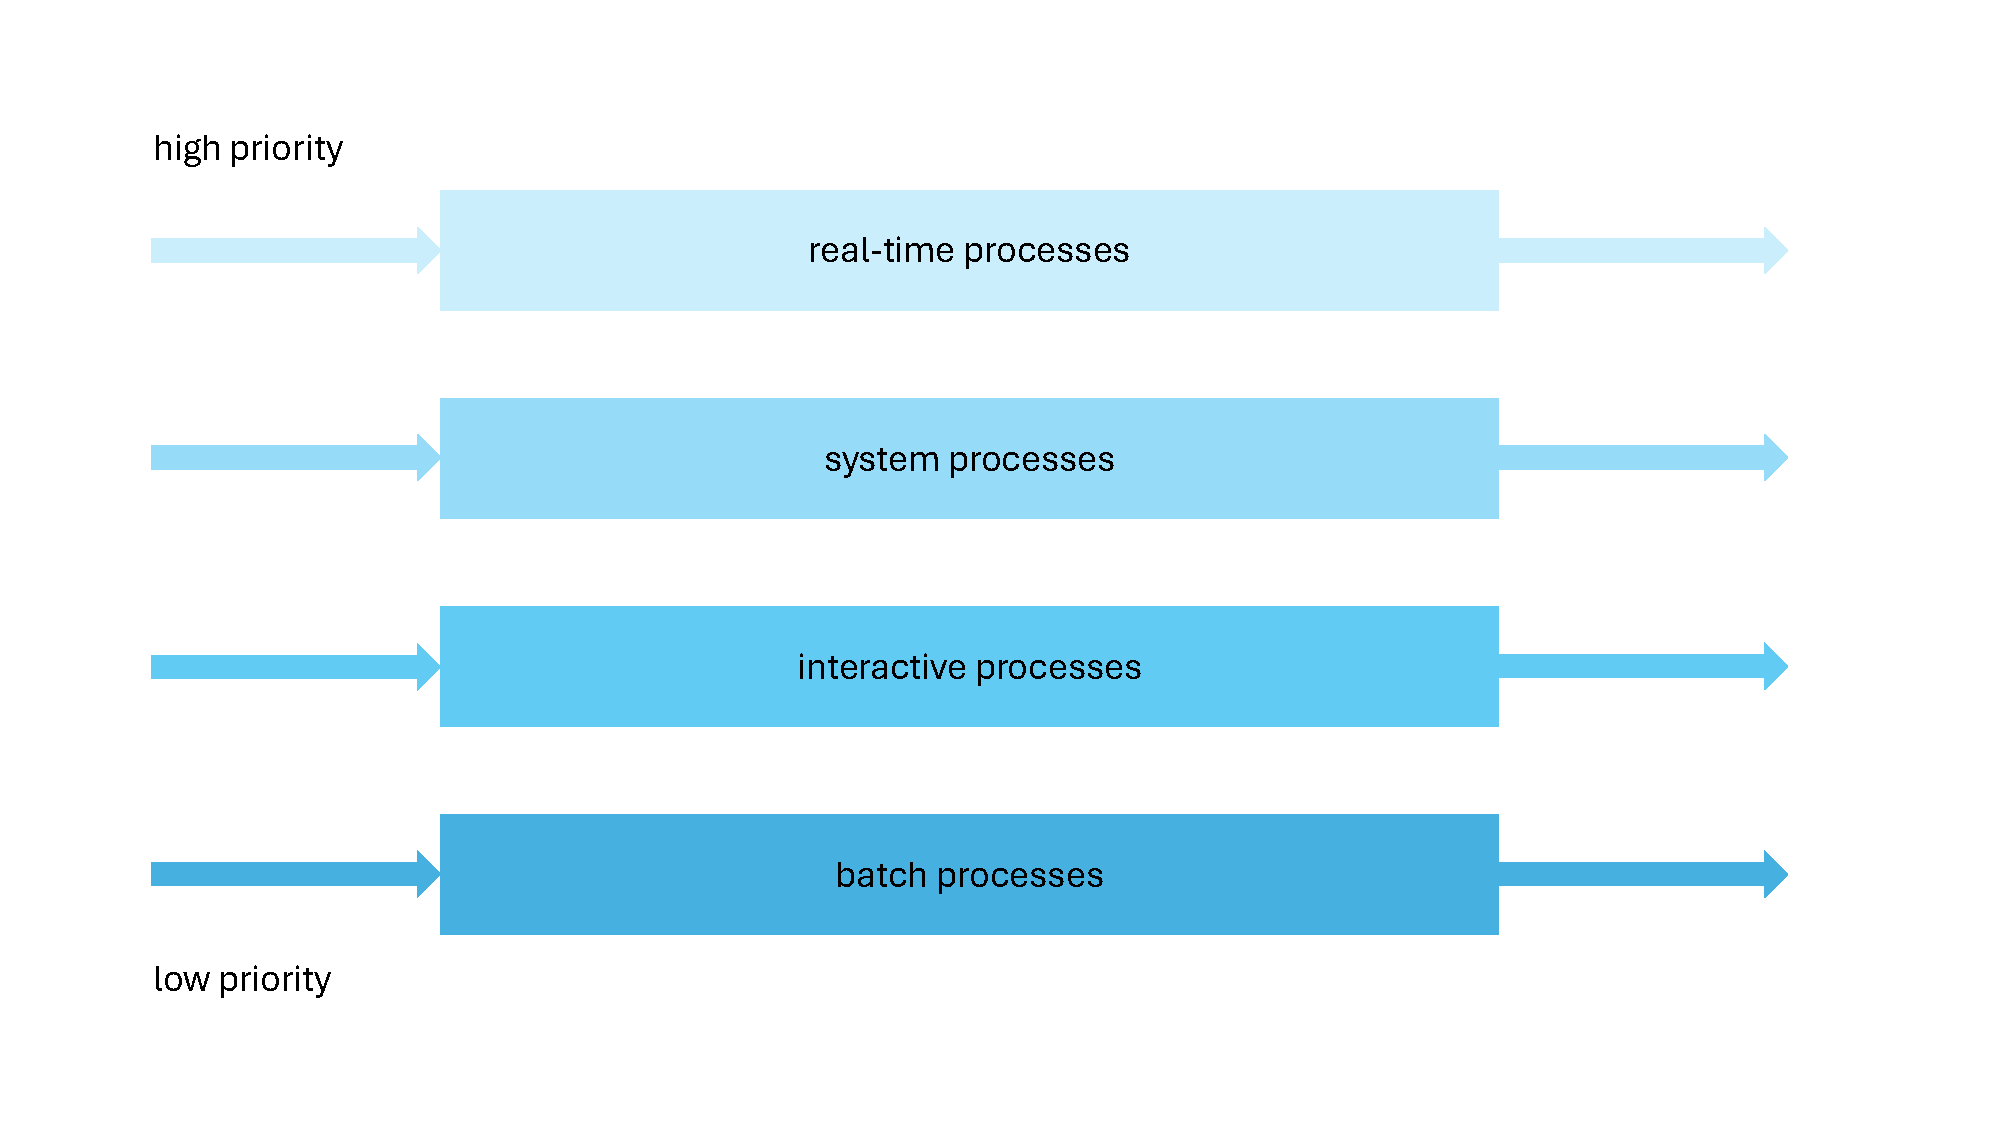
\includegraphics[width=\linewidth]{img/mlq.pdf}
	\caption{Darstellung des \ac{MLQ}-Schedulings mit mehreren Warteschlangen \cite[S.215]{Silberschatz.2019}}
	\label{fig:mlq_queues}
\end{figure}

Das Multilevel Queue Scheduling Verfahren bietet aufgrund seiner erweiterten Komplexität gegenüber herkömmlichen deutlich einfacheren Verfahren einige Vorteile, aber auch Nachteile. So ist positiv zu bemerken, dass die Reaktionszeit des Systems durch die effizientere Ressourcenallokation reduziert werden kann und die Nutzererfahrung durch die schnellere Abarbeitung von interaktiven Prozessen verbessert wird. Des Weiterem kann mit diesem Verfahren unter den richtigen Umständen der Durchsatz gesteigert werden und das System ggf. auch Prozesse unterschiedlicher Schlangen gleichzeitig ausführen, welches zu der Effizienz des Systems beiträgt. Negativ zu betrachten sind hingegen die erhöhte Komplexität beim Design eines effizienten Systems sowie der zusätzliche Arbeitsaufwand zur Verwaltung der mehreren Warteschlangen untereinander, welcher die Performance des Systems wiederum lindern kann. Ein weiteres Problem ist das „Verhungern“ von Prozessen in einer Warteschlange mit niedrigerer Priorität, welches auftreten kann, wenn zu viele, große Prozesse in anderen Schlangen zuerst abgearbeitet werden müssen.
Um diesem Nachteilen des „Verhungerns“ von Prozessen entgegenzuwirken, gibt es Weiterentwicklungen der einfachen Multilevel Queue wie beispielsweise das heute verbreitete Multilevel Feedback Queue Verfahren. Hier sind die Prozesse nicht komplett fest einer Warteschlange zugeordnet, sondern können auch zu einem späteren Zeitpunkt noch in eine andere Schlange verschoben werden. Dies hilft dabei, dass das System besser auf die Bearbeitungszeiten der Prozesse reagieren kann und keine Prozesse vernachlässigt werden.
%könnte man ggf. noch im Detail ausführen, falls wir mehr Text brauchen


%%%%
%Der zentrale Vorteil von \ac{MLQ} liegt in dessen Flexibilität und Effizienz bei der Behandlung verschiedener Prozesstypen. Beispielsweise können Systemprozesse, interaktive Prozesse und Batch-Prozesse in verschiedenen Warteschlangen mit entsprechenden Prioritäten und Scheduling-Strategien verwaltet werden. Hierdurch wird eine bessere Anpassung an die Anforderungen spezifischer Prozesstypen erreicht, was zu einer verbesserten Gesamtleistung des Systems führt. % Tanenbaum und Bos (2014) 

%Ein Nachteil von \ac{MLQ} liegt allerdings in seiner Komplexität, sowohl in der Implementierung als auch im Management. Die korrekte Einordnung von Prozessen in Warteschlangen und die Auswahl geeigneter Scheduling-Algorithmen für jede Warteschlange erfordern sorgfältige Planung und ständige Anpassung. Eine nachteilige Auswahl und Konfiguration dieser Algorithmen kann zu einem erhöhten Overhead führen und die Systemeffizienz negativ beeinträchtigen. % Stallings (2012)

%Trotz dieser Herausforderungen ist \ac{MLQ} ein beliebter Scheduling Algorithmus in Betriebssystemen, insbesondere dort, wo eine Vielzahl unterschiedlicher Prozesse und Anforderungen effizient verwaltet werden muss.

%\textit{Referenzen:}
%\begin{itemize}
%	\item Silberschatz, A., Galvin, P. B., \& Gagne, G. (2018). Operating System Concepts. Wiley.
%	\item Tanenbaum, A. S., \& Bos, H. (2014). Modern Operating Systems. Pearson.
%	\item Stallings, W. (2012). Operating Systems: Internals and Design Principles. Prentice Hall.
%\end{itemize}




% !TEX root =  master.tex
\chapter{Performance Analyse}
Die richtige Auswahl der zuvor vorgestellten Scheduling Algorithmen ist ein essenzieller Bestandteil, um die Gesamtleistung und Reaktionsfähigkeit des Systems zu optimieren. Die zentrale Herausforderung hierbei ist die begrenzte Verfügbarkeit der \ac{CPU}, da diese zu einem Zeitpunkt stets nur einen Prozess ausführen kann. Während OS Scheduling Algorithmen versuchen den Einsatz der \ac{CPU} zu optimieren, indem diese entscheiden welcher Prozess als nächstes bearbeitet werden soll, muss stets der am besten geeignete Algorithmus ausgewählt werden. Daher wird sich in diesem Kapitel mit den wichtigsten Metriken zur Auswahl der Algorithmen beschäftigt, um im anschließenden Abschnitt \ac{FCFS}, Round Robin und \ac{MLQ} basierend auf Simulationsergebnissen miteinander zu vergleichen.
% !TEX root =  master.tex

\section{Metriken}
Um unterschiedliche Scheduling Algorithmen wie \ac{FCFS}, Round Robin oder \ac{MLQ} bezüglich ihrer Performance und somit ihrer Eignung für Anwendungsgebiete vergleichen zu können, ist es möglich diverse Metriken zu verwenden. Die Auswahl ist abhängig vom jeweiligen Anwendungsgebiet, beispielsweise wird in interaktiven Systemen eine geringe Antwortzeit priorisiert, während bei Batch-Processing-Systemen eine niedrige Ausführungszeit von höherer Relevanz ist \autocite{thombare_efficient_2016}. Im Folgenden werden häufig genutzte Metriken erklärt, welche im Anschluss für den quantitativen Vergleich verwendet werden.


\textbf{\ac{CPU}-Auslastung (\ac{CPU} Utilization)}: Diese Metrik gibt an, wie effektiv die \ac{CPU} genutzt wird. Eine hohe \ac{CPU}-Auslastung bedeutet, dass die \ac{CPU} aktiv an Prozessen arbeitet, was ein Indikator auf eine effiziente Nutzung der Ressourcen ist \autocite{pemasinghe_comparison_2022}. Die folgende Formel \ref{met:cpu} berechnet den prozentualen Wert der \ac{CPU}-Auslastung, zu welcher die \ac{CPU} Prozesse bearbeitet, bezogen auf die gesamte Beobachtungszeit.
\begin{equation}
	\textit{CPU-Auslastung} = \frac{\textit{Gesamtaktive Zeit}}{\textit{Gesamtbeobachtungszeit}} \times 100
	\label{met:cpu}
\end{equation}


\textbf{Durchsatz (Throughput)}: Der Durchsatz misst die Anzahl der Prozesse, welche in einer zuvor definierten Zeiteinheit vollständig abgearbeitet werden. Hierbei bedeutet ein höherer Durchsatz eine effizientere Verarbeitung von Prozessen durch das System  \autocite{pemasinghe_comparison_2022}. Bei vollständiger \ac{CPU}-Auslastung ist der Durchsatz bei unterschiedlichen Algorithmen konstant, sofern von einem möglichen Overhead durch Context Switches abgesehen wird. Die Formel \ref{met:throughput} berechnet den Durchsatz als Anzahl der Prozesse, die pro Zeiteinheit abgeschlossen werden.
\begin{equation}
	\textit{Durchsatz} = \frac{\textit{Anzahl\ der\ Prozesse}}{\textit{Zeiteinheit}}
	\label{met:throughput}
\end{equation}


\textbf{Durchschnittliche Antwortzeit (Response Time)}: Die Antwortzeit berechnet die Zeit vom Beginn eines Prozesses bis zur ersten Antwort. Diese Metrik ist besonders wichtig in interaktiven Systemen, wo eine schnelle Reaktion auf Benutzereingaben erforderlich ist  \autocite{pemasinghe_comparison_2022}. In Formel \ref{met:responsetime} wird die Berechnung der Wartezeit dargestellt, welche die durchschnittliche Antwortzeit über alle \( n \) Prozesse ist.
\begin{equation}
	\textit{Durchschnittliche Antwortzeit} = \frac{\sum_{i=1}^{n} (\textit{Startzeit}_{i} - \textit{Ankunftszeit}_{i})}{n}
	\label{met:responsetime}
\end{equation}


\textbf{Durchschnittliche Wartezeit (Waiting Time)}: Die Wartezeit eines Prozesses ist die Gesamtzeit, welche dieser in der Warteschlange verbringt, bevor er Zugang zur \ac{CPU} erhält  \autocite{pemasinghe_comparison_2022}. Niedrigere Wartezeiten sind meist erstrebenswert, da es sich hierdurch für gewöhnlich um ein reaktionsfähigeres System handelt. In folgender Formel \ref{met:waitingtime} ist \( n \) die Anzahl der Prozesse, und die Wartezeit wird als Durchschnitt der Zeit berechnet, die jeder Prozess vom Ankunftszeitpunkt bis zum Start der Ausführung wartet.
\begin{equation}
	\textit{Durchschnittliche Wartezeit} = \frac{\sum_{i=1}^{n} ((\textit{Abschlusszeit}_{i} - \textit{Ankunftszeit}_{i}) - \textit{Bearbeitungszeit}_{i})}{n}
	\label{met:waitingtime}
\end{equation}


\textbf{Durchschnittliche Umlaufzeit (Turnaround Time)}: Bei der Umlaufzeit handelt es sich um die gesamte Dauer vom Start eines Prozesses bis zu dessen Abschluss \autocite{pemasinghe_comparison_2022}. Es wird somit sowohl die Wartezeit, als auch die Bearbeitungszeit berücksichtigt, weshalb ein umfassenderer Vergleich bezüglich der Effizienz von Scheduling Algorithmen möglich ist. Die Ausführungszeit wird als durchschnittliche Gesamtzeit berechnet, die ein Prozess vom Ankunftszeitpunkt bis zum Abschluss benötigt.
\begin{equation}
	\textit{Durchschnittliche Umlaufzeit} = \frac{\sum_{i=1}^{n} (\textit{Abschlusszeit}_{i} - \textit{Ankunftszeit}_{i})}{n}
	\label{met:turnaroundtime}
\end{equation}


\textbf{Fairness}: Die Metrik der Fairness misst, wie gleichmäßig die \ac{CPU}-Zeit zwischen den verschiedenen Prozessen aufgeteilt wird. Ein fairer Scheduling-Algorithmus stellt sicher, dass kein Prozess übermäßig bevorzugt oder benachteiligt wird \autocite{haldar_fairness_1991}. Es handelt sich hierbei um eine qualitative Metrik, weshalb es in der Literatur keine festgelegte Berechnung hierfür gibt. Stattdessen wird die Fairness oft durch die Analyse der Verteilung von den Wartezeiten über die verschiedenen Prozesse hinweg bewertet, beispielsweise durch die Berechnung der Standardabweichung. Folgende Formel \ref{met:fairness} stellt die beispielhafte Berechnung hiervon dar, wobei dies nicht als universeller Weg angesehen wird.
\begin{equation}
	\textit{Fairness} = \sqrt{\frac{\sum_{i=1}^{n} (\textit{Wartezeit Prozess}_{i} - \textit{durchschnittliche Wartezeit})^2}{n}}
	\label{met:fairness}
\end{equation}

% !TEX root =  master.tex


\section{Simulationsergebnisse}
- Erst kurz den Aufbau beschreiben. 
- Nutze einfach gleich so 10k an Prozesse und erkläre wie diese Prozesse erstellt wurden --> damit es nachvollziehbar sind. 
- Dann kann ich erst eine Abbildung der Boxplots mitaufnehmen und zusätzlich noch eine Tabelle wo alles drinnen steht. 
- Dann erklären was die bedeuten und was für Insights man ziehen kann. 
- Am Ende noch eine Bestätigung, dass das mit der allgemeinen Literatur übereinstimmt

% !TEX root =  master.tex
\chapter{Anwendungsgebiete}
Innerhalb dieses Kapitels werden wird auf konkrete Anwendungsgebiete der zuvor genannten OS-Scheduling Algorithmen eingegangen. Da diese Algorithmen auch außerhalb von Betriebssystemen einen zentrale Rolle spielen, werden auch Beispiele solcher Anwendungsgebiete aufgenommen.

% !TEX root =  master.tex

\section{Innerhalb von Betriebssystemen}
Ein häufiges Anwendungsgebiet von \ac{FCFS} ist für Aufgaben der Batch-Verarbeitung, da hierbei der Convoy-Effekt nicht entscheidend ist. Ein klassisches Beispiel ist das Druckmanagement in frühen Betriebssystemen, wo Druckaufträge in der Reihenfolge ihres Eintreffens abgearbeitet werden.  %\textit{Referenz:} Silberschatz, Galvin, and Gagne. \textit{Operating System Concepts}. 9th ed., John Wiley \& Sons, 2012.

Round Robin hingegen ist ein weit verbreiteter Scheduling Algorithmus in zeitkritischen Betriebssystemen. Ein Beispiel hierfür ist das Thread-Scheduling in Unix-basierten Systemen, bei dem jedem Thread eine feste Zeitscheibe zugeteilt wird. %\textit{Referenz:} Tanenbaum, Andrew S., and Bos, Herbert. \textit{Modern Operating Systems}. 4th ed., Pearson, 2014.

\ac{MLQ} wird in modernen Betriebssystemen wie Linux angewendet, um Prozesse basierend auf ihrer Priorität zu ordnen, wobei systemkritische Prozesse höher priorisiert werden als Benutzerprozesse. % \textit{Referenz:} Love, Robert. \textit{Linux Kernel Development}. 3rd ed., Addison-Wesley Professional, 2010.

In modernen Betriebssystemen ist der Aufbau der Prozessverwaltung und Anwendung von Scheduling Algorithmen ein komplexes Thema, welches in der Praxis eine Vielzahl von Anforderungen erfüllen muss. Die hier vorgestellten Algorithmen sind nur ein kleiner Ausschnitt der Vielzahl von Scheduling Algorithmen, die in modernen Betriebssystemen zum Einsatz kommen.

\subsubsection{Windows}
Windows verwendet beispielsweise 7 Prioritätsstufen.
Prozesse können sich selbst die folgenden Stufen zuweisen:
\begin{multicols}{3}
    \begin{itemize}[noitemsep]
        \item IDLE
        \item BELOW NORMAL
        \item NORMAL
        \item ABOVE NORMAL
        \item HIGH
        \item REALTIME
    \end{itemize}
\end{multicols}

Innerhalb eines Prozesses können die einzelnen Threads dann jeweils 7 Prioritätsebenen haben, die die Threads untereinander sortieren:
\begin{multicols}{3}
    \begin{itemize}[noitemsep]
        \item IDLE
        \item LOWEST
        \item BELOW NORMAL
        \item NORMAL
        \item ABOVE NORMAL
        \item HIGHEST
        \item CRITICAL
    \end{itemize}
\end{multicols}

Windows verwendet beide Prioritätszuweisungen um dem Thread eine Basispriorität zu geben, die zwischen 0 und 31 liegt \autocite{KarlBridgeMicrosoft.2023}.

\subsubsection{MacOS}
Mit der Einführung der neuen M-Serie Prozessoren unterteilt Apple die Prozessorkerne in Performance- und Effizienzkerne. Die Performancekerne sind für rechenintensive Aufgaben und die Effizienzkerne für weniger rechenintensive Aufgaben zuständig.
% !TEX root =  master.tex

\section{Außerhalb von Betriebssystemen}
\ac{FCFS} wird in zahlreichen Gebieten verwendet, insbesondere bei Prozessen die eine schwierige Digitalisierbarkeit aufweisen. Beispielsweise wird \ac{FCFS} in der Industrieautomatisierung, insbesondere in der Steuerung von Fertigungsstraßen, verwendet, bei welcher Aufträge in der Reihenfolge ihres Eingangs bearbeitet werden. % \textit{Referenz:} Groover, Mikell P. \textit{Automation, Production Systems, and Computer-Integrated Manufacturing}. 4th ed., Prentice Hall, 2016.
Auch in Bereichen fernab von Computern und Industrie wird \ac{FCFS} in alltäglichen Situationen eingesetzt. Ob die Warteschlange an der Kasse im Supermarkt, die Patientenabfertigung im Krankenhaus in der Notaufnahme oder auch der Essensausgabe in der Kantine. 

Ein bekanntes Anwendungsgebiet von Round Robin ist die Telekommunikation. Hierbei wird Round Robin für die Paketvermittlung und Lastverteilung in Netzwerkroutern eingesetzt. Ein Beispiel ist die Verteilung von Netzwerkbandbreite in Cisco-Routern. %\textit{Referenz:} Kurose, James F., and Ross, Keith W. \textit{Computer Networking: A Top-Down Approach}. 7th ed., Pearson, 2016.
Darüber hinaus wird Round Robin in der Luftfahrtindustrie für die Flugzeugbodenabfertigung eingesetzt, um eine faire und effiziente Zuteilung von Abfertigungsdiensten zu gewährleisten. %\textit{Referenz:} Wells, Alexander T., and Young, Seth B. \textit{Airport Planning \& Management}. 6th ed., McGraw-Hill Education, 2011.

\ac{MLQ} findet beispielsweise Anwendung in Cloud-Computing-Umgebungen wie AWS oder Google Cloud, wo verschiedene Instanzen oder Services in getrennten Warteschlangen basierend auf SLAs verwaltet werden. %\textit{Referenz:} Rhoton, John. \textit{Cloud Computing Explained: Implementation Handbook for Enterprises}. 2nd ed., Recursive Press, 2013.





% Fazit und Ausblick
%% !TEX root =  master.tex
\chapter{Zusammenfassung}

\nocite{*}

Dieses Kapitel enthält die Zusammenfassung der Arbeit mit Fazit und Ausblick.

\section{Fazit}

...

\section{Ausblick}

...


%%%%%%%%%%%%%%%%%%%%%%%%%%%%%%%%%%%

%%%%%%%%%%%%%%%%%%%%%%%%%%%%%%%%%%%
% ANHÄNGE
%
% @stud: einzelne Anhänge bearbeiten und eigene Anhänge hier einfügen 
%        die nachfolgenden Zeilen deaktivieren, wenn keine Anhänge verwendet werden
%
\initializeAppendix
% !TEX root =  master.tex
\chapter{Ressourcen}
Der vollständige Quellcode ist über folgenden GitHub Link erreichbar: \linebreak
\href{https://github.com/echtermeyer/OS-Scheduling-Algorithms-Comparison}{https://github.com/echtermeyer/OS-Scheduling-Algorithms-Comparison}

Das Video kann auf Youtube unter folgendem Link gefunden werden: \linebreak
\href{https://youtu.be/9bVAGvbL8Gc}{https://youtu.be/9bVAGvbL8Gc}

%% !TEX root =  master.tex
\chapter{Beispiel-Anhang: Noch ein Testanhang}
nochmal: lipsum ...

%%%%%%%%%%%%%%%%%%%%%%%%%%%%%%%%%%%

\singlespacing

%%%%%%%%%%%%%%%%%%%%%%%%%%%%%%%%%%%
% LITERATURVERZEICHNIS
% @stud: Literaturverzeichnis in Datei bibliography.bib anpassen. 
%
% Alternative zu Verwendung von \initializeBibliography: Citavi ...
% (dann \initializeBibliography auskommentieren und eigenes LaTex Coding verwenden)
%
\initializeBibliography
%%%%%%%%%%%%%%%%%%%%%%%%%%%%%%%%%%%

%%%%%%%%%%%%%%%%%%%%%%%%%%%%%%%%%%%
% INDEX
% @stud: ggf. Index auskommentieren, wenn nicht benötigt
%
\addcontentsline{toc}{chapter}{Index}
\printindex

\end{document}
